\documentclass[11pt, oneside]{article}      % use "amsart" instead of "article" for AMSLaTeX format
\usepackage{geometry}                       % See geometry.pdf to learn the layout options. There are lots.
\geometry{letterpaper}                          % ... or a4paper or a5paper or ... 
%\geometry{landscape}                       % Activate for rotated page geometry
%\usepackage[parfill]{parskip}          % Activate to begin paragraphs with an empty line rather than an indent
\usepackage{graphicx}               % Use pdf, png, jpg, or eps§ with pdflatex; use eps in DVI mode
                                % TeX will automatically convert eps --> pdf in pdflatex        
\usepackage{amssymb}
\usepackage[capposition=top]{floatrow}
\usepackage{subcaption}
\usepackage{algpseudocode}
\usepackage{algorithm}

%SetFonts

%SetFonts

% To compile bibliography, in Terminal
% $ latex filename
% $ biber filename
% $ latex filename

% Additional Packages
% Bibliography Package:
\usepackage[% comment spaces as biblatex sometimes dislikes them a lot
        natbib=true,% just this for natbib compatibility - don't load natbib itself
        bibstyle=authoryear,%
        citestyle=authoryear-comp,%
        %hyperref=true,%
        citetracker=true,
        backend=biber,%
        maxbibnames=1,%
        firstinits=true,%
        uniquename=init,%
        maxcitenames=2,%
        maxbibnames=10,
        parentracker=true,%
        url=false,%
        doi=false,%
        isbn=false,%
        eprint=false,%
       % backref=true,%
            ]  {biblatex}\addbibresource{mz_bib.bib}
\AtEveryCitekey{\ifciteseen{}{\defcounter{maxnames}{99}}}

\usepackage{amsmath}
\linespread{1.6}
\usepackage{comment}

\begin{document}
\begin{titlepage}
    \begin{center}
        \vspace*{1cm}
        
        \Huge
        \textbf{Our Grid's Second Wind:}
        
        \vspace{0.5cm}
        \Large
        The effect of increased wind generation on wholesale electricity prices
        
        
        \vspace{1.5cm}
        \textbf{Michelle J. Zheng}
        
        \vfill
        
        \large
        Senior Honors Thesis\\
        Brown University Economics Department\\
        April 18, 2016\\
        \vspace{0.8cm}
        
        
        Advisor:\\
        Anja Sautmann\\
        \par
        Acknowledgements:\\
        Jerry Elmer, Christopher Geissler, James Fine
        
    \end{center}
\end{titlepage}


\section{Introduction}

Wind energy is a rapidly growing resource, already providing 4.5\% of electricity in the US and projected to supply up to 35\% by 2050. Relying only on the strength of the wind to power its electricity-generating turbines, wind power has no need for fuel. While there are still operational and maintenance costs, the lack of marginal fuel costs makes wind power highly competitive at the margin with other more established types of generation, such as coal, natural gas, hydropower, and nuclear. Furthermore, it is virtually greenhouse gas emission-free and does not pollute nor consume resources, making it a key technology in decarbonizing the grid and meeting climate goals (US Department of Energy, 2015).

One way in which wind energy reaches end users is through the purchase of bulk electric power systems. In the United States, these are non-profit organizations appointed by the Federal Energy Regulatory Commission (FERC) called Independent System Operators (ISOs). They are responsible for coordinating the flow of energy across the electrical grid, fairly administering electricity markets, facilitating non-market electricity purchase contracts, and planning the power grid to ensure that it can meet demand. They are funded by collecting service fees from market buyers and sellers at the minimum level required to cover costs. Their markets manage 60\% of the nation's electricity with the goal of procuring the supply necessary to meet demand for the entire system, by allowing individual generators to submit bids detailing the quantity and price at which their resource can supply to the market. Energy is procured from these generators through a least-cost purchasing rule known as the merit order, which accepts energy bids in increasing cost order until demand is met. This energy is then transmitted throughout the grid, reaching homes and businesses throughout the ISO's territory in order to meet demand (US Energy Information Administration, 2011).

In this paper, I quantify the ability of wind to reduce prices for consumers, asking: how does the quantity of wind generation being bid in competitive electricity markets affect the wholesale price of electricity? Bid in by wind generators at \$0.00 marginal cost, wind energy should decrease prices at levels varying by 1) the quantity of wind added to the market, 2) the level of demand, and 3) the marginal costs and quantities of other resources on the market. Assuming perfectly inelastic demand and leaving out the effect of the exit of other firms in the long run, I estimate the impact of increased wind penetration under different quantity, demand, and resource mix scenarios by simulating the market mechanism using historical market data and evaluating the price changes that result. I look specifically for this effect at the day-ahead market administered by the New England ISO (ISO-NE), which accounts for about 30-40\% of the energy procured in this region of 14 million customers.


\section{Background}
The process of balancing supply and demand on an ISO's territory is complex. Below are discussions of key terms, parties, and processes.

\subsection{Independent System Operators (ISOs)}
Created by Orders Nos. 888/899 by the FERC, ISOs are independent nonprofit corporations responsible for ensuring that supply (electricity generation) matches demand (system load) in their territories at all times. In their real-time and day-ahead market-based procurement processes, they tell generators when to turn on and off via a market process known as the merit order in order to achieve this balance. The remainder of the grid's energy is settled in longer term contracts, which are non-market purchase agreements between specific buyers and sellers. Revenue also flows to generators through the capacity market, which allows rarely-activated generators to remain in the market to offer supply during high demand and emergency hours, ensuring grid reliability -- an ISO's highest priority. ISOs handle the bulk procurement of electricity, while customer-facing utilities and businesses then purchase and distribute from the ISO to end users \parencite{isonewengland2016roles}.

\subsection{Merit Order and the Bid Curve}
Wholesale electricity markets are organized as auctions. During each auction period (generally at the hourly or sub-hourly level), generators bid in prices and quantities at which they can supply electricity to the grid. They also provide other information on their startup and shutdown speed (``ramping rate'') and costs. The ISO then accepts some of the bids offered based on a procurement mechanism called the merit order, calling only upon the accepted bids to run and supply energy during the bidding period and requiring that rejected bids turn or remain off. [22]

Merit order describes the ordering of all bids over all generators from least to greatest cost for each settlement period on an ISO market, with the the resources of greatest ``merit'' appearing first at the bottom of the ordering. This creates the bid curve, which represents supply in the market. It is a commonly utilized bidding mechanism also known as a multi-unit discriminatory auction, used in refinancing auctions coordinated by central banks [20]. As demand increases, price increases as well due to the merit order. Due to the nature of different resources' generation costs, costs along the merit ordering tend to grow exponentially, though this depends on the the types of resources making up the bid curve. Generally, renewables and nuclear bid in at or below \$0/MW due to their low marginal costs of production. Depending on the market and time of year, fossil fuel resources such as gas, oil, and coal may appear in different price ranges. The last, marginal generator to be activated (the generator with the greatest cost of generation accepted within the period before demand is met) sets the price paid to all generators that fall below the marginal generator on the bid curve. This is known as the clearing price \parencite{robertethiervamsichadalavada2009}. Generators are required to bid at their marginal costs of production, and are barred from conducting strategic behavior (see section below on the Internal Market Monitor). A more in-depth discussion of the merit order mechanism appears later on as a preface to the methodology.

\subsection{ISO New England (ISO-NE)}
Established in 1997, ISO-NE procures energy for the region spanning Connecticut, Rhode Island, Massachusetts, Vermont, New Hampshire, and the majority of Maine. Serving 14 million people, it purchases energy from 350 generators and holds about 31,000 MW of generating capacity \parencite{isonewengland2016keygrid}. As of January 2016, its resource mix is comprised of 41.3\% gas, 25.1 nuclear, 7.7\% renewables (with 1.7\% coming from wind), 6.4\% hydro, 3.6\% coal, and 1.8\% oil \parencite{isonewengland2016keygrid}.  However, this is posed to change drastically: 42\% of newly proposed projects in the region as of 2015 are wind generation, and 57\% are natural gas. Coal and oil generation have already declined greatly, slowly replaced by natural gas through the 2000s. Nuclear power is also expected to wane, due to political disfavor and the increasing costs of operation and maintenance as plants age \parencite{isonewengland2015outlook}. Energy procurement by ISO-NE is comprised of approximately 60\% contracts, 30-40\% day-ahead, and 0-10\% real-time as of the beginning of 2016; we focus on the day-ahead market as there is little data available on the contract market and does not abide by the merit order process, and the real-time market procures a negligible percent of system supply \parencite{jerryelmer2015interview}. Additionally, prices in the real-time and day-ahead markets do not differ by much, with a correlation of  0.9340 and nearly-identical means and standard deviations (see appendix figure 1).

ISO-NE has played a particularly important role in making renewable energy competitive in its markets, providing evidence against the criticism of renewable resources as intermittent and thus unreliable. This has been done in two main ways: making renewables dispatchable, and allowing for negative price offers. 

A dispatchable resource is allowed to submit bids and set clearing prices in the ISO's markets. Dispatchable resources meet the following requirements: 1) they have telemetry (constant electronic communication) with the ISO, 2) the ISO can rely on accurate five-minute-ahead forecasts on generation output, and 3) the ISO has algorithms that allow it to dispatch renewable generators at levels controlled to five-minute granularity \parencite{jerryelmer2014}. By assisting wind generators in achieving the first two conditions and taking the initiative to implement the third, ISO-NE can now treat wind as a dispatchable resource, which comes with the ability to set the clearing price. Though this has not yet had large implications with wind currently making up less than 2\% of resources, wind will only grow in prominence in the coming years, increasing the likelihood of wind-dictated clearing prices at greater levels of penetration \parencite{conservationlawfoundation2014}.

Additionally, resources can bid in at negative prices. This is allowed for the purpose of avoiding imbalances during low demand hours (typically in the early morning) by letting generators signal that they would be willing to pay to produce electricity in order to avoid the costs associated with shutdown and start-up, or else quickly curtail their generation in response to the price signal without requiring ISO administrative action. This benefits wind, which must operate when the wind blows (or else curtail generation at some cost) and often has non-market sources of revenue (such as tax credits and other renewable generation incentive schemes, depending on the state of renewable energy policy at the time) that allow it to operate economically even under a negative clearing price. Thus, wind can ensure that it will be activated in any scenario \parencite{isonewengland2015outlook}.

\subsection{Generation mix of ISO-NE}
Electricity demand in New England is largely met by gas and nuclear generation. [data1] Although the region historically relied, to a greater extent, on coal and oil, this has changed as environmental policies, market forces, and the aging of plants have pushed it out of the mix. Coal and oil still make up 28\% of the region's capacity. However, they act largely as crucial reserve generation to meet spikes in demand or the price of natural gas and only supplied 2\% of demand in 2014, kept in the market mainly via payments from the capacity market. Nuclear generation is also expected to leave the market as prices have dropped with the introduction of more natural gas, which has made it more difficult for nuclear plants to recover medium term costs, such as those of compliance with safety regulations and refueling \parencite{christophergeissler2016}. Natural gas and wind are expected to dominate the resource mix of the future, making up 57\% and 42\% of new generator proposals submitted to the ISO as of January 2015 \parencite{isonewengland2015outlook}. 

\begin{figure}
    \centering
    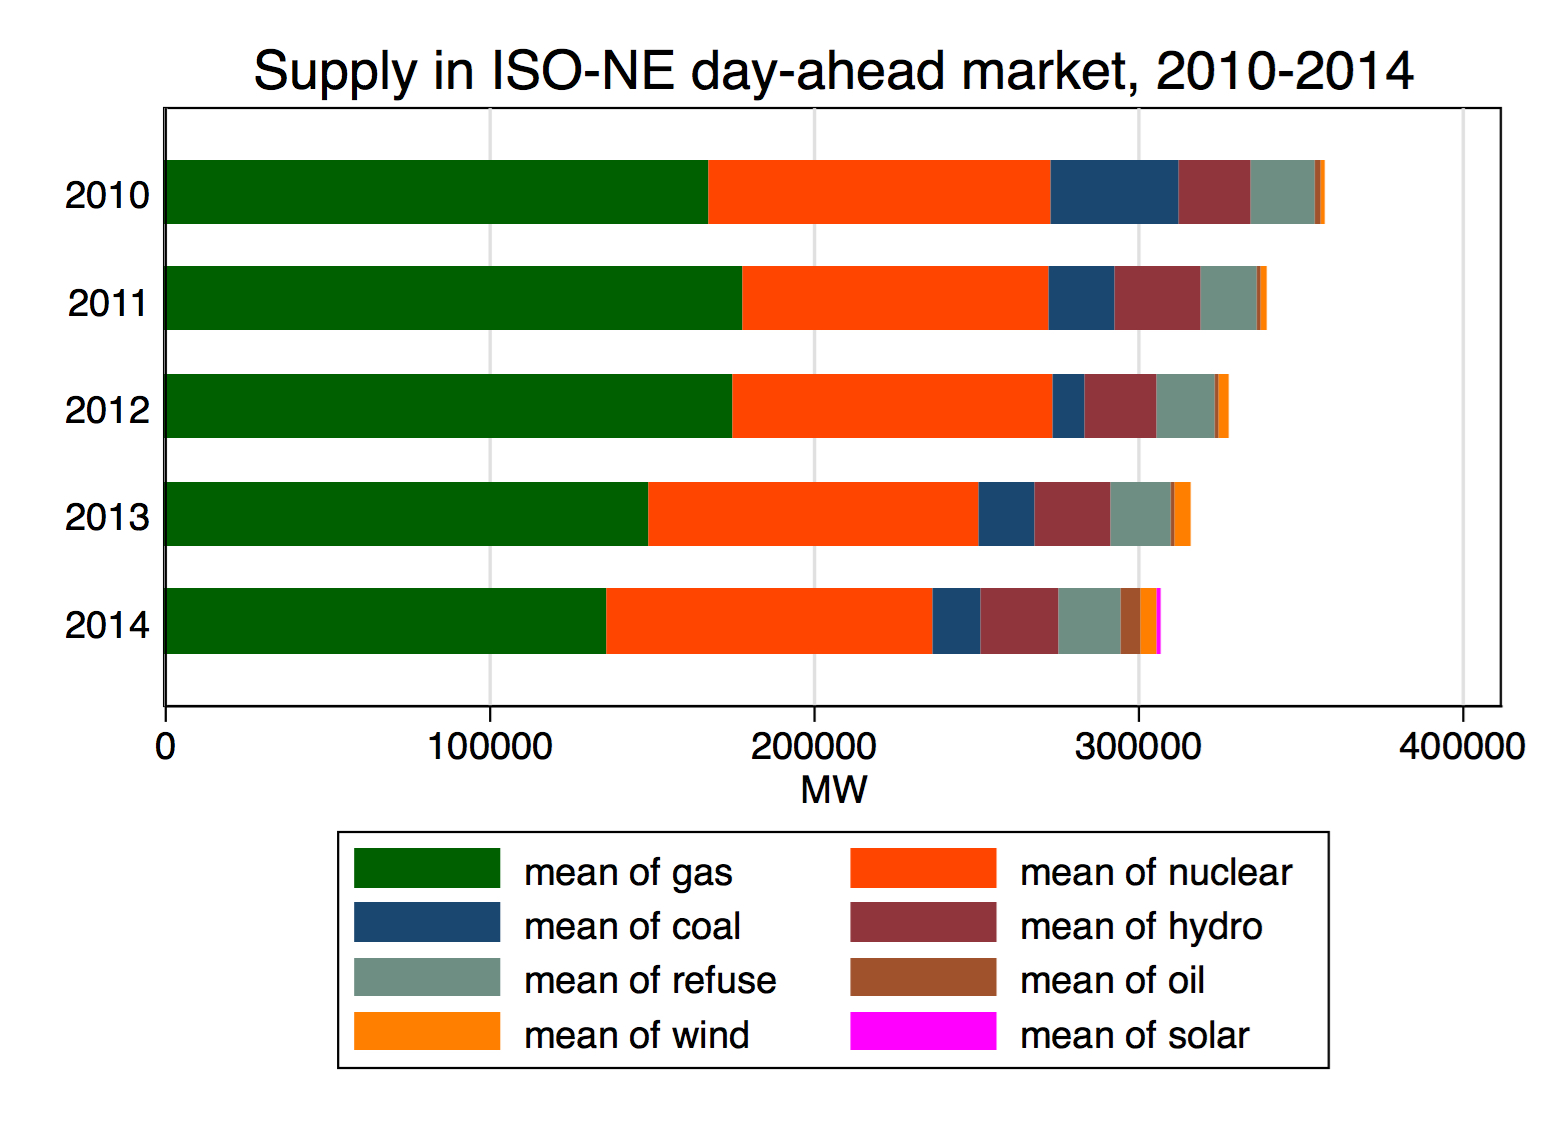
\includegraphics[width=12cm]{figures/rmix_yearly.jpg}
    \floatfoot{Figure 1: The ISO-NE system is dominated by gas and nuclear generation, with remaining resources making up fewer than 25\% of supply.}
\end{figure}

Demand and the generation mix vary seasonally (see appendix figure 2 for summary statistics). In the winter, natural gas makes up a smaller fraction of the generation mix despite higher system demand. This is due to increased demand for natural gas for household heating, which drives up its price and makes it less competitive on the electricity market - an increase in coal use during winters results \parencite{isonewengland2015outlook}. Scarcity and price spikes have been particularly driven in the region by natural gas pipeline capacity bottlenecks \parencite{usenergyinformationadministration2013}. However, the highest demand of the year occurs in the summer, when electricity is used for cooling. Clearing price has been known to spike to levels nearly 20 times the average during the hottest days of the year, as caused by the sharp exponential increase in price that characterizes rarely-activated generators at the rightmost side of the bid curve. [data1]

\begin{figure}
    \centering
    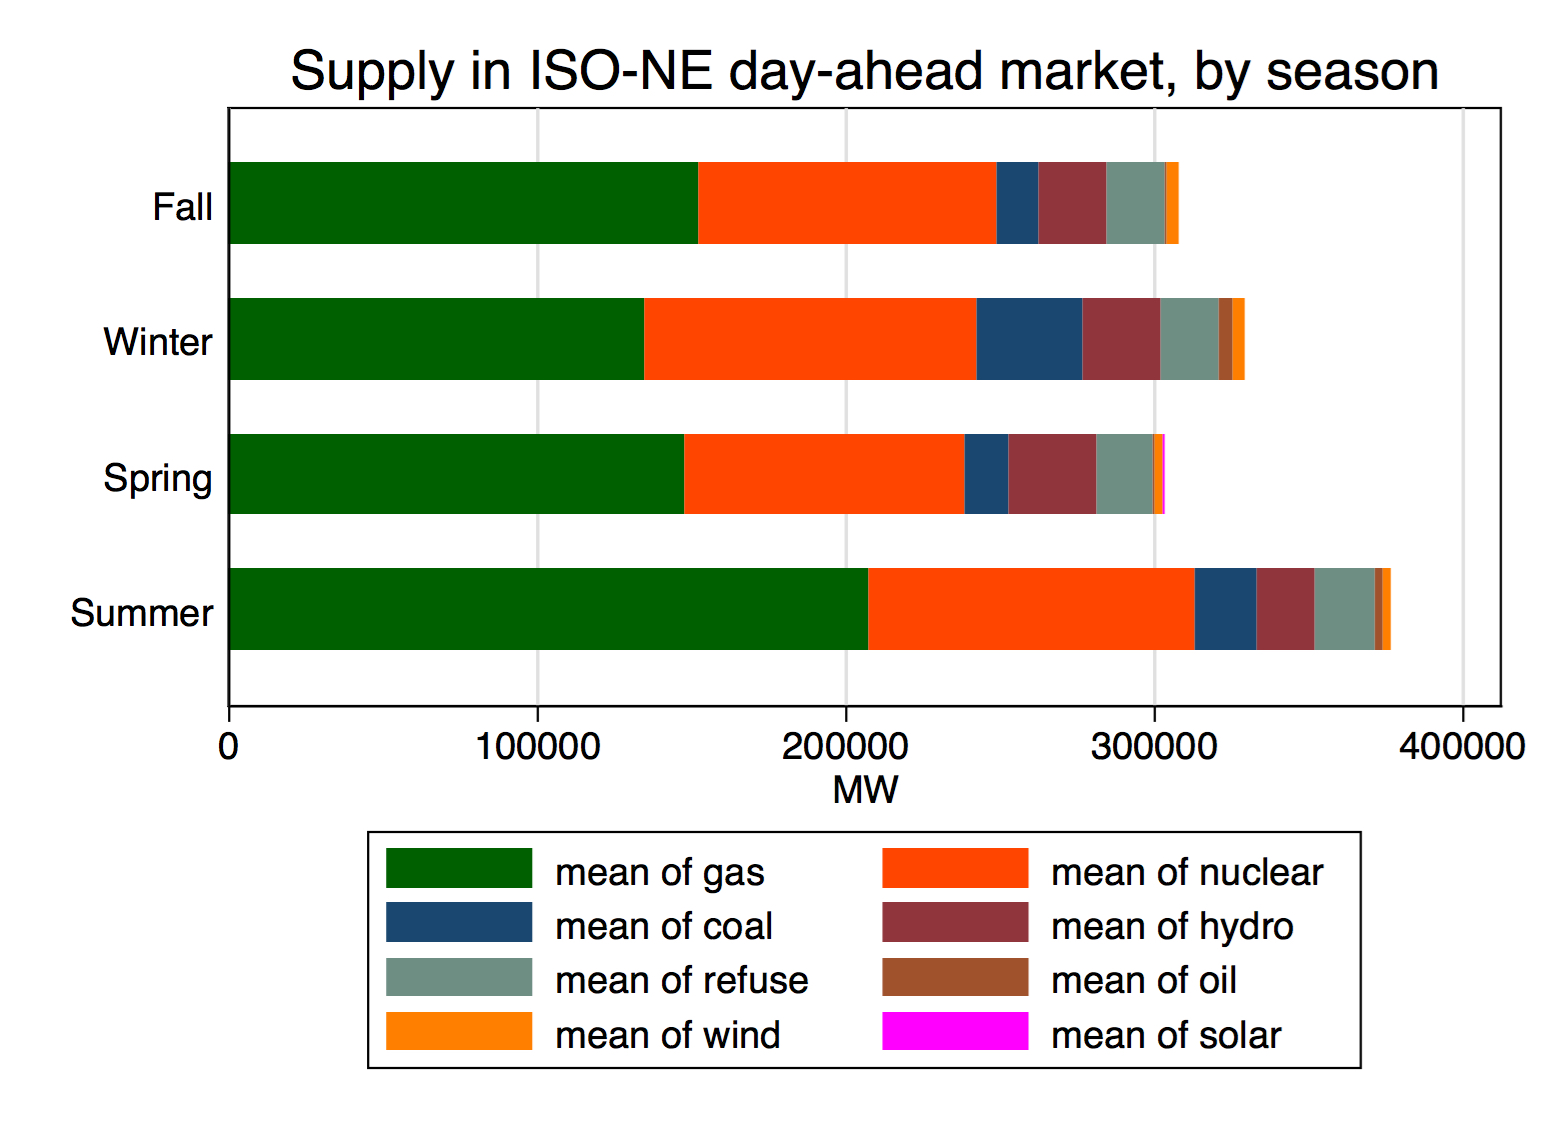
\includegraphics[width=12cm]{figures/rmix_seasonal.jpg}
    \floatfoot{Figure 2: Coal and natural gas exhibit significant seasonal variation.}
\end{figure}

\subsection{The Internal Market Monitor (IMM)}
The Internal Market Monitor (IMM) at ISO-NE is a department functioning independently of the ISO, responsible ``for the daily detection and mitigation of the effects of any anti-competitive behavior in the wholesale markets or market products.'' The IMM responds to activities manipulating market prices, conditions, or rules with legal action and financial penalties \parencite{isonewengland2016imm}. Most generators are required to submit offers into the day-ahead market that do not exceed their marginal costs; their costs and capacity are monitored by the IMM. Thus, though quantity generated may vary based on factors such as timing of maintenance and unexpected shutdowns, generators are not allowed to freely withhold capacity \parencite{christophergeissler2016}. The function of the IMM is crucial to upholding the effectiveness of the merit order process in procuring energy at least cost, as it deters generators from bidding strategically in response to the offers of other market participants. For example, in the absence of regulatory oversight, non-wind generators could easily predict the output of wind via forecasts that are publicly announced (or otherwise predictable from weather forecasts) before the bidding period and withdraw quantity in order to artificially increase prices (see section VI for a more detailed discussion).



\section{Literature}
While many have estimated the effects of wind generation on electricity market prices, none have simulated the direct price impact of additional units of wind as a counterfactual to historical data. Below, I discuss existing estimations of wind's impact on prices, the effect of the energy mix on this impact, attempts to structurally model the supply and demand curves in these markets, and potential engineering constraints that may dampen the price suppressant effect of wind.

 The impact of wind and other renewable resource generation on electricity prices is known as the merit order effect, and has been estimated by a number of different researchers with data from markets around the world. Jonsson, Pinson, and Madsen (2009) demonstrated the effect of wind on Danish spot prices in the Nord Pool Elspot market (which is far more wind-saturated than ISO-NE with wind comprising 20\% of generating capacity). Using wind power forecasts as a proxy for generation magnitude, they showed a shift in the mean price towards zero as wind penetration increased, with 2\% of periods of over 40\% wind penetration demonstrating a spot price of \$0.00. [lit1] Ketterer (2014) showed that the impact of wind energy on prices via the merit order effect is more strongly negative during the day than night, depends on the generation mix and flexibility of conventional capacity, and has decreased over time in German markets. [lit2] Cl�, Cataldi, and Zoppoli (2015) use a regression model similar to the one I use in estimating the relative effects of different resources on the clearing price; their model controls for the effects of demand, natural gas price, and time-based fixed effects to show the price decreasing effects of additional wind and solar generation on the Italian power market. [lit8]

The merit order effect varies by level of wind penetration, accuracy of forecast, and whether curtailment (when the system operator forces a resource to stop contributing to system supply in the case of overproduction) is allowed in a market. Mart�nez-Anido, Brinkman, and Hodge (2016) show that volatility increases and price decreases as wind penetration increases, with more volatility appearing at more granular market timescales (eg. five minute vs. hourly). Though I do not take into account forecast accuracy or curtailment, I do expand upon the effect of different levels of natural gas supply on wind's effect on price as they suggest should be explored in future research.

The price effects of additional wind generation depend on the existing energy mix. O'Flaherty, Riordan, O'Neill, and Ahern (2014) show that increased wind penetration in Ireland has little impact on average prices because of the prevalence of imported gas generation from the UK, which comprises 48\% of supply and generally function as the price setting marginal fuel. [lit3] Mart�nez-Anido and Hodge (2014) note that increasing wind penetration has its greatest effect on the generation mix via reducing gas and oil generation, the most common marginal fuel on the bid curve. However, the use of these resources increases as the accuracy of wind forecast decreases; in the case that wind generation falls short of forecasted levels, gas and oil are often called upon to meet the gap as fast-ramping generators that can quickly activate at relatively low cost. [lit7] Following this literature, I later take the level of gas generation into account when estimating the impact of additional wind generation in my simulation.

Structural models are commonly used, due to the clear relationships between underlying market factors and prices that can be represented as a classic supply-and-demand problem. Boogert and Dupont (2007) attempt to estimate both the supply and demand curves in a manner able to generate price spikes, improving upon past models by creating a ``hockey-stick'' supply curve reflecting the sudden exponential increase in prices after a certain quantity supplied, and a demand curve reflecting the effects of seasonality and temperature. [lit6] \textcite{michaelcoulonsamhowison2008} describe the high correlation between the price of natural gas and market prices in both New England and the PJM market (serving the Mid-Atlantic states), noting its price-setting power as a fuel in the middle of the bid curve. They develop a structural model for spot prices based on underlying factors of the market such as demand and generation capacity, and apply it to the same bid curve model that I use to determine the effect of movements in clusters of bids (due to changing underlying fuel costs) on price. Their methodology emphasizes the importance of capturing the effects of many parameters at once due to the complexity of electricity markets and the determination of clearing price by a substantial number of factors on both the supply and demand sides. [lit4] 

Others note the potential effects of engineering considerations of wind's effect on price. Troy (2010) suggests that increasing the penetration of variable power resources like wind and solar, which produce energy according to uncontrollable weather factors, can lead to issues with baseload plants (which provide an underlying reserve of energy to guarantee the viability of the power system in the case that variable output falls) due to increased cycling, or startup and shutdown, of the plants, leading to increased maintenance costs and failures. This cancels out some of the effect of fuel cost savings by the introduction of zero fuel cost variable output resources. [lit5] Though the effects do not express themselves directly through electricity markets (rather, through non-marginal venues such as the capacity market), they should be considered in system-wide analyses of wind impact on price. In terms of wind's effect on transmission across the grid, Mart�nez-Anido and Hodge (2014) find no major impacts on transmission-level system operations, even in the absence of an ISO's ability to view the operations of power plants at an individual utility-scale level. However, they qualify that this may only hold for low penetrations of wind. [lit7]

\section{The merit order procurement mechanism}
The merit order procurement mechanism is the process used by the ISO to accept the supply needed to meet demand at least cost. [22] It minimizes the cost of procuring electricity by accepting bids of price and quantity in least cost order until demand is met. This can be expressed as follows:

\begin{algorithm}
\caption{Merit order procurement}
\begin{algorithmic}
\State $bids\gets {(p_1,q_1), ..., (p_n,q_n)}$\Comment{List of bids in increasing cost order of (price, quantity)}
\State $demand\gets d$
\State $supply\gets 0$
\For{($p_i$, $q_i$) in range[1,n]}
\State $supply\gets supply+q_i$
\If{supply $\geq$ demand}
\State $clearingPrice\gets p_i$
\State \Return clearingPrice
\EndIf
\EndFor
\end{algorithmic}
\end{algorithm}

The merit order holds for the vast majority of hours, though it is occasionally overridden if other grid constraints must be met. For example, if demand sharply spikes between hours, the next cheapest resource may be ignored in favor of a different resource that can activate more quickly to provide electricity in time for the next hour. Another case is of transmission constraints: the next cheapest resource may be ignored if it is located in a place on the grid that is not capable of providing electricity to meet demand appearing in a different part of the grid due to transmission constraints (when electrical lines are physically unable to transmit electricity between two locations). However, cases like these are non-dominant and unpredictable with the data available; thus, I assume in my market simulation that such constraints do not occur. Future work should relax this assumption, as wind generation tends to take place in areas farther away from the sources of greatest demand (i.e. offshore or in less populated rural areas), suggesting there may be a correlation between wind generation and increased overriding of the merit order unless additional transmission infrastructure is built to counteract this potential effect.

At its most simplified, the supply curve formed by the ordering of bids forms an exponential curve, with clearing price corresponding to the intersection of supply with a fixed level of demand. The drivers of the exponential shape of the supply curve and the magnitude of demand are discussed below.

\begin{figure}
    \centering
    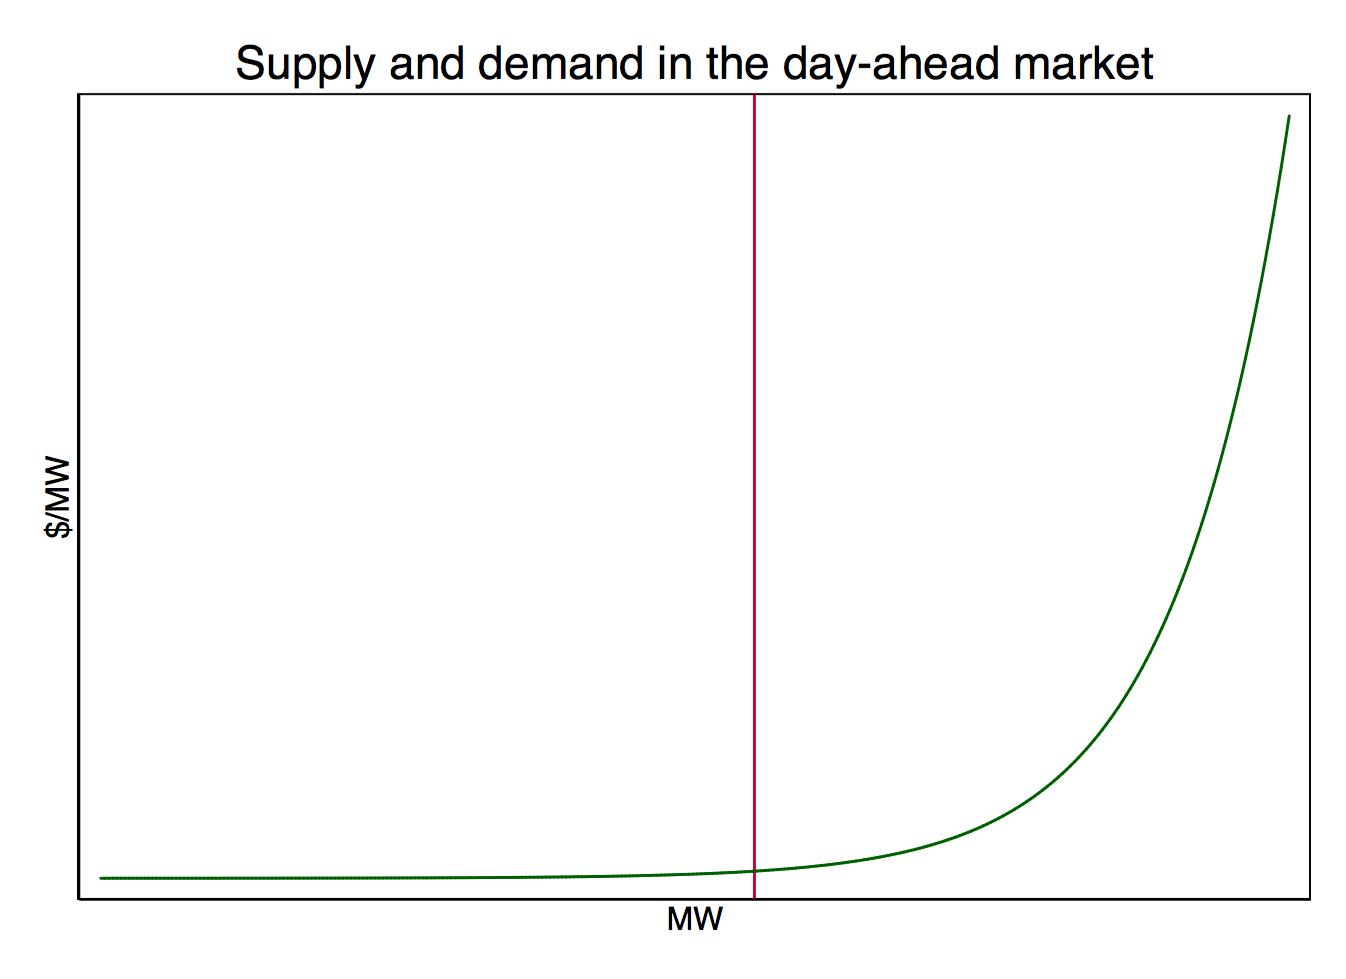
\includegraphics[width=12cm]{figures/simple_supply_demand.jpg}
    \floatfoot{Figure 3: A schematic representation of supply and demand.}
\end{figure}

\subsection{Demand}
In the short run, demand is determined largely independently of supply and price, driven by factors such as the season, time of day, day of the week, weather, and efficiency of electrical appliances and buildings. It is relatively inelastic to changes in price, since there are often no substitutes for electrical power. This changes slightly in the long run, when consumers can make more long-term changes in their consumption levels in response to price (such as buying more energy-efficient fixtures, improving building insulation). For example, elasticity of demand of residential electricity price in New England is estimated to be about -0.192 in the short run, and -0.325 in the long run \parencite{m.a.bernsteinj.griffin2006}. Economic growth has been a large driving factor in the past, but this effect has waned as growth in GDP has increasingly decoupled from growth in electricity demand. [21] However, the effect of demand on price is clear: the higher the demand, the higher the resulting clearing price. Seasonal fluctuations in demand and price arise from the use of heating and cooling appliances in the summer and winter (see figure 4). 

\begin{figure}
    \centering
    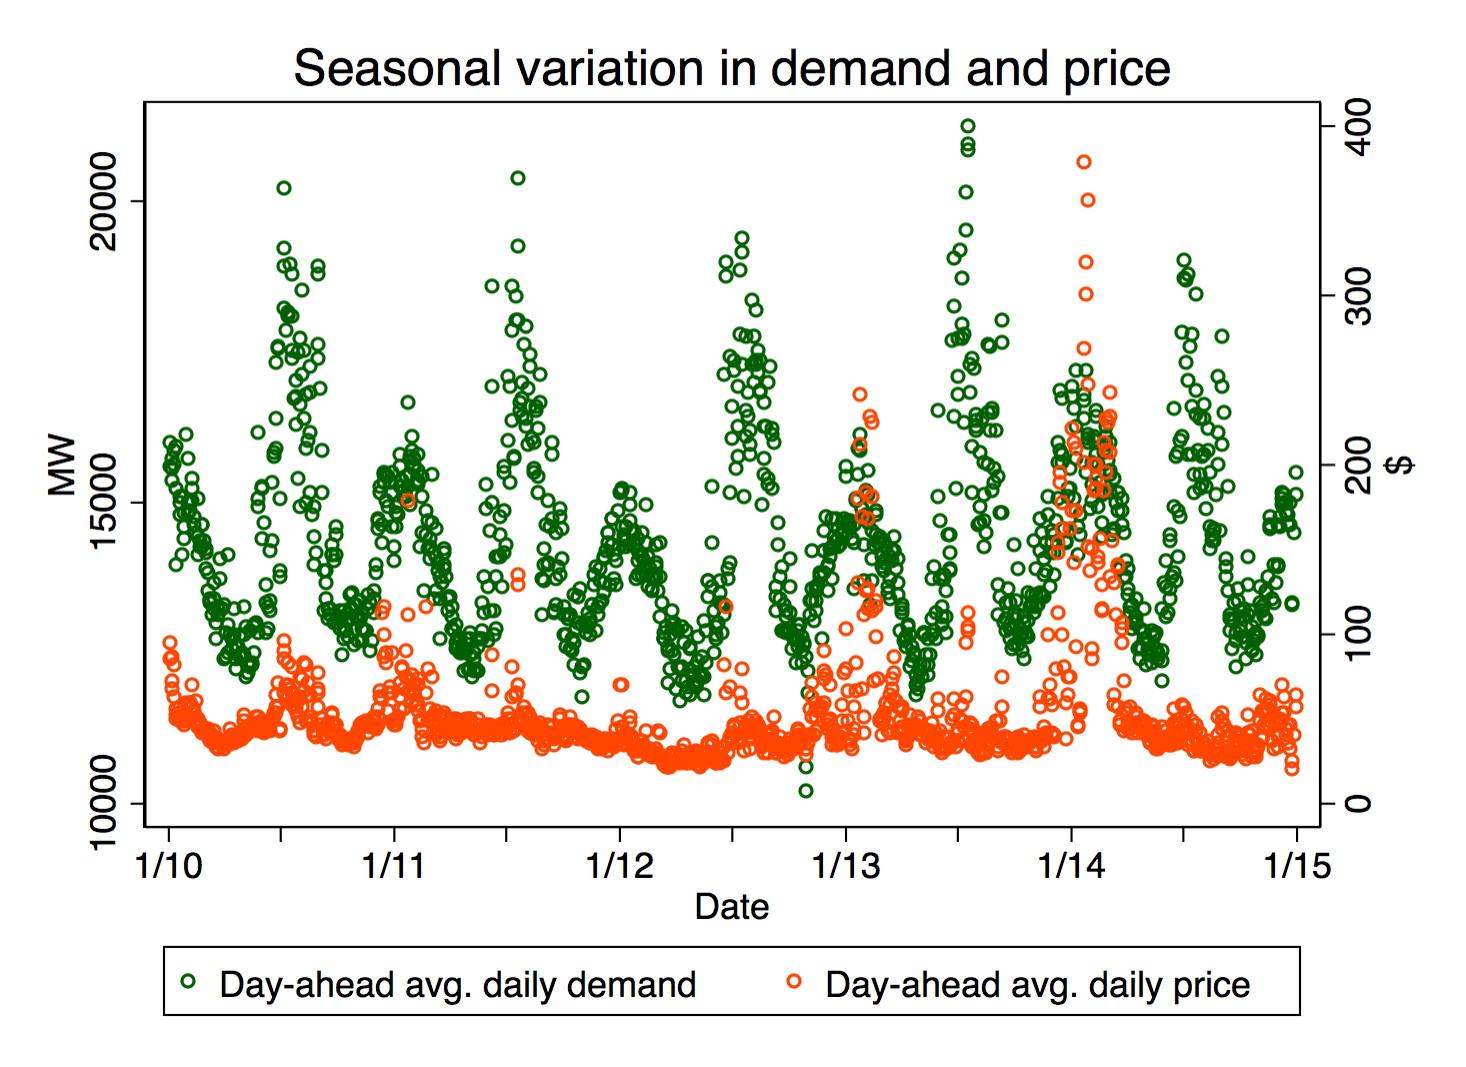
\includegraphics[width=12cm]{figures/demand-price.jpg}
    \floatfoot{Figure 4: Demand and price tend to spike concurrently.}
\end{figure}

Fluctuations also occur throughout the day, with additional variation by season. Summer demand peaks in the afternoon around 3 PM as mid-afternoon temperatures cause a peak in the use of cooling devices, whereas peaks in other seasons occur as people wake up in the morning and prepare for their day, and then later as they return home from work. The intensity of mid-afternoon summer peaks make summer the highest demand season, with winter coming in next due to fewer sunlight hours and more time spent indoors. Spring and fall exhibit similar load patterns. Demand is always lowest at night and in the early morning when people are not awake. 

\begin{figure}
    \centering
    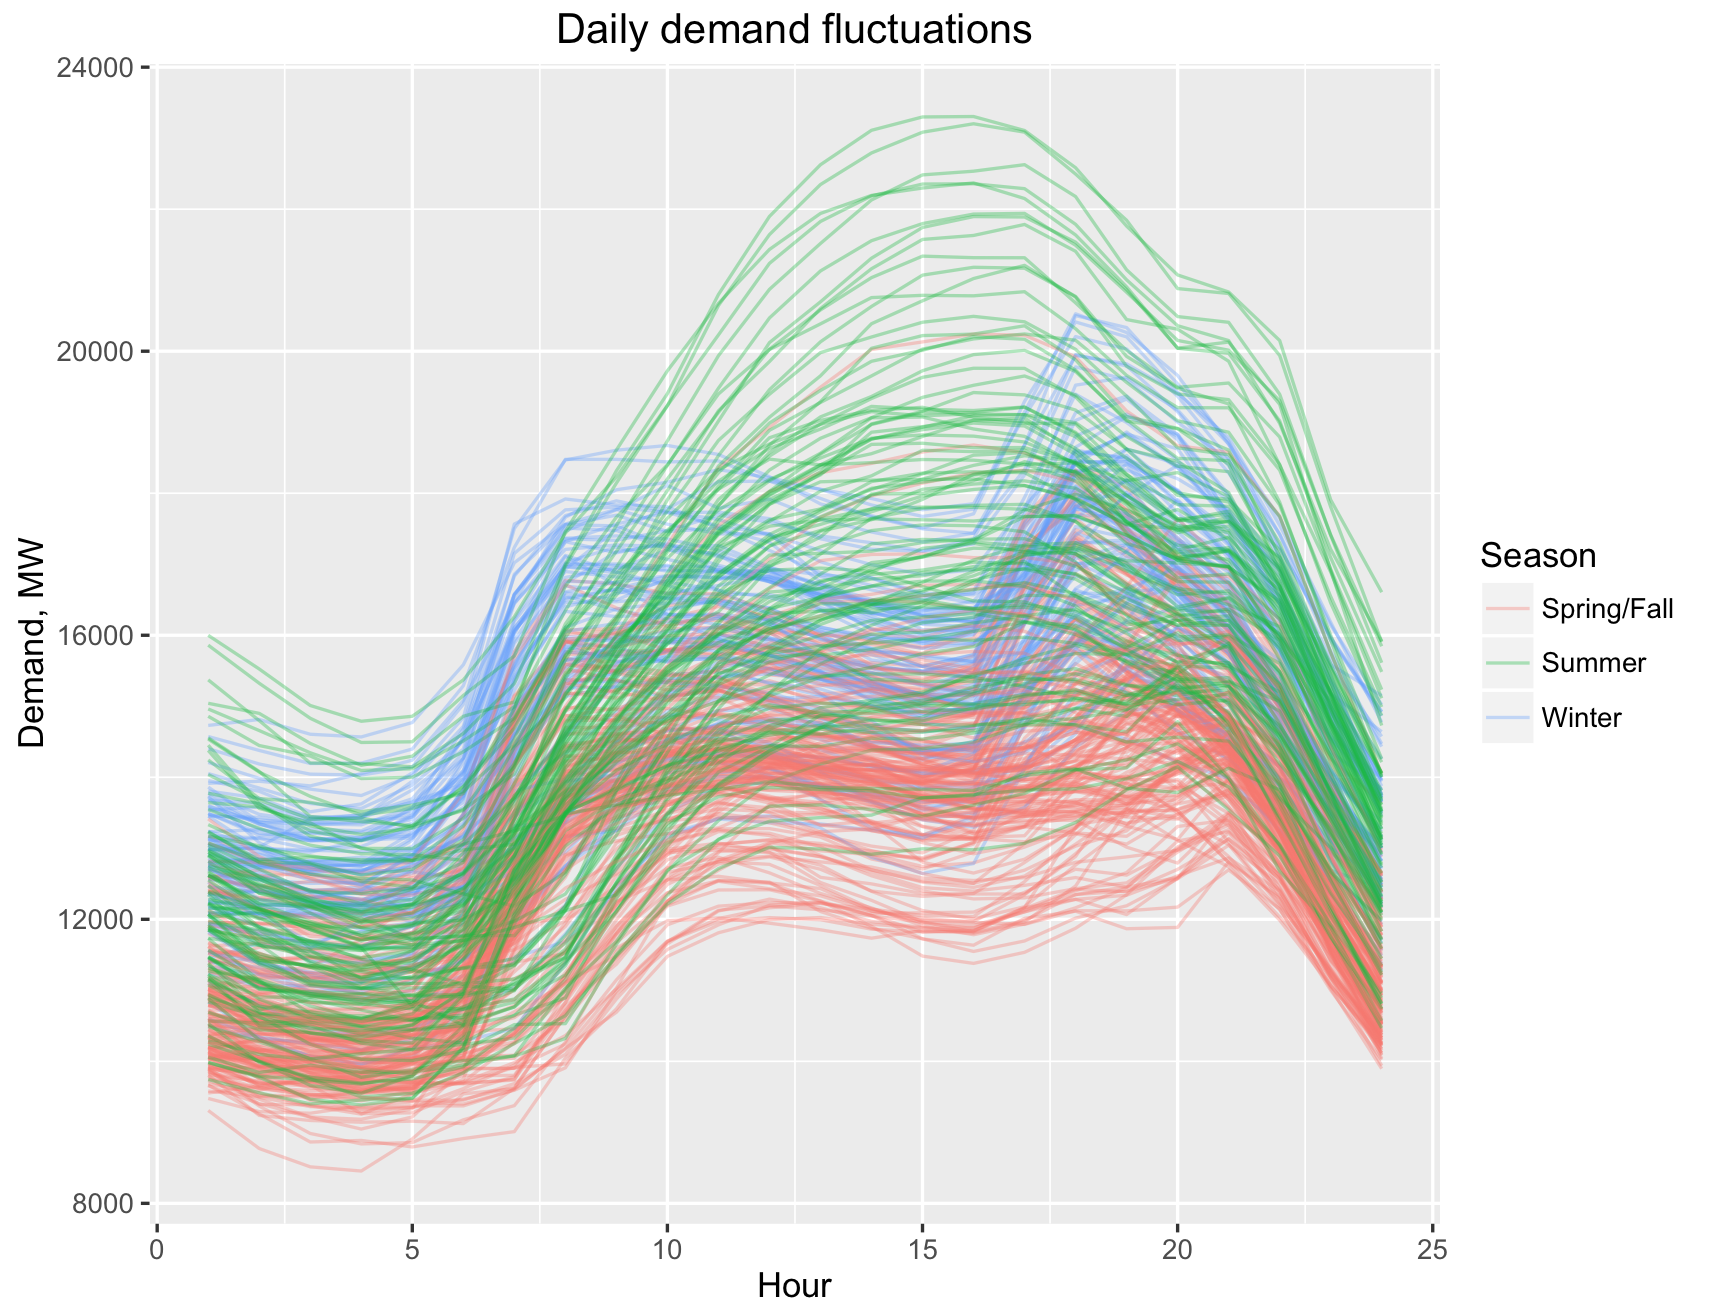
\includegraphics[width=12cm]{figures/daily_fluc.png}
    \floatfoot{Figure 5: Daily demand patterns vary seasonally.}
\end{figure}

\subsection{Supply}
Putting the bids of all generators in increasing price order results in the construction of the bid curve, which provides an useful visual representation of price variation in a market. The exponential behavior of the bid curve can be seen in the figure below, as constructed from day-ahead offer data taken from ISO-NE's system on January 1st, 2014 at 9 AM. This exponential shape is the result of 1) bids from rarely-activated, more expensive reserve generators and 2) expensive higher segment bids offered by generators with marginal costs varying by quantity supplied.

The red line indicates the demand of the hour, which is 13,847.9 MW and crosses with the supply curve at \$174.61, the clearing price. All generators bidding at or below this price will clear demand and be paid this amount for each MW bid during the hour, while generators above are not activated. This exponential shape explains the appearance of price spikes during hours of abnormally high demand, since generators at the far right of the curve exhibit significantly higher costs. It also suggests that prices remain relatively stable when demand remains between 10,000-20,000 MW (which it generally does), as the slope of that middle range is relatively gradual.

\begin{figure}
    \centering
    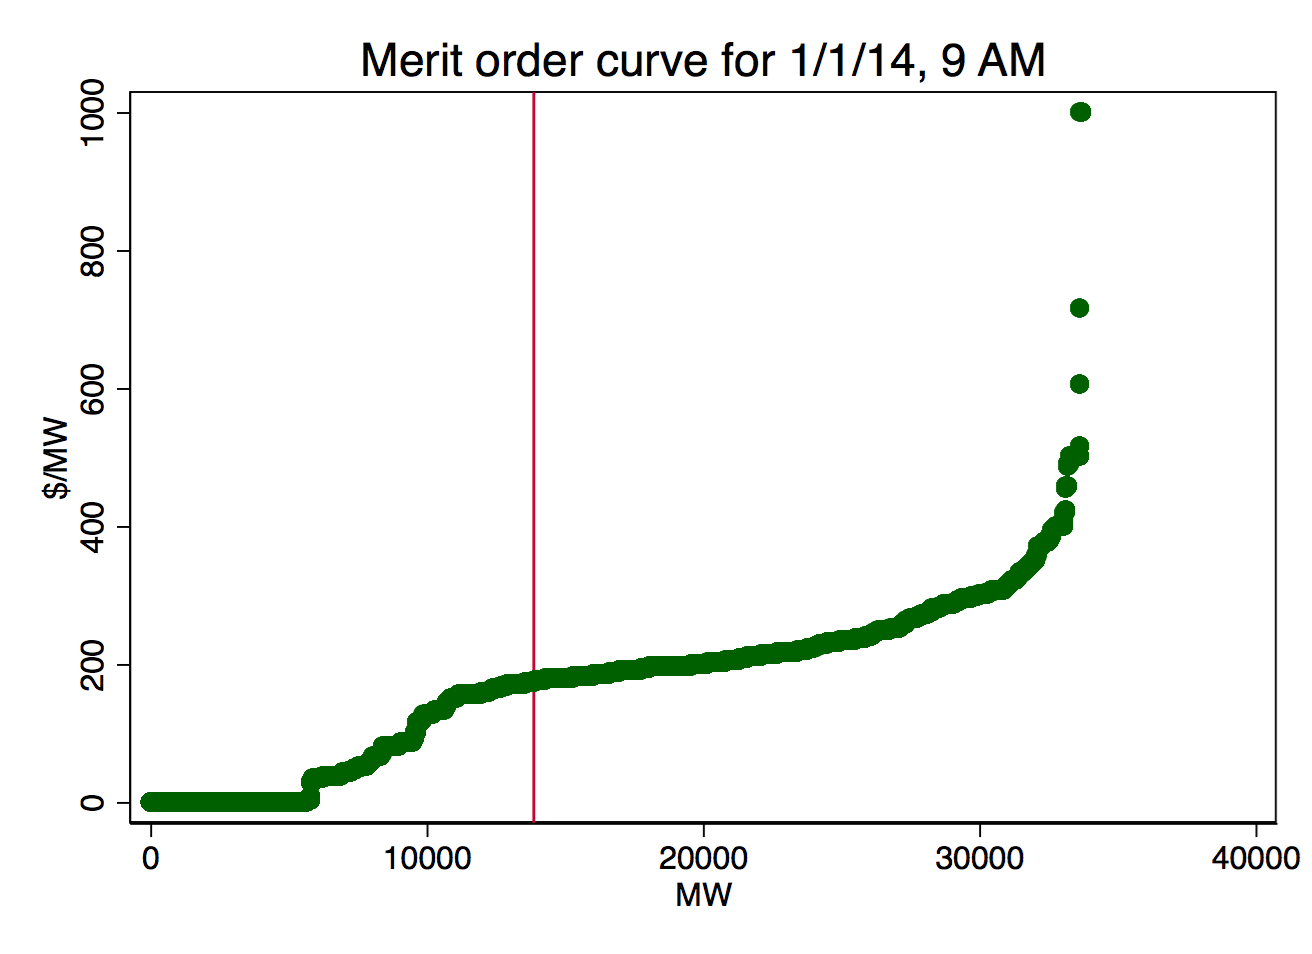
\includegraphics[width=12cm]{figures/bid2014}
    \floatfoot{Figure 6: The bid curve displays an exponential shape.}
\end{figure}

A look at the same day and hour in 2010 shows that the resource mix has changed over the years. This earlier date displays a more gradual slope upwards where the 2014 date shows a sharper increase between 6,000-10,000 MW. This smoother curve may have been due to the presence of more nuclear generation, which provides relatively low to no marginal cost electricity, and volatility in the price of natural gas, which directly alters marginal costs for generators and adjusts the slope of the gas-dominated middle section of the curve.

\begin{figure}
    \centering
    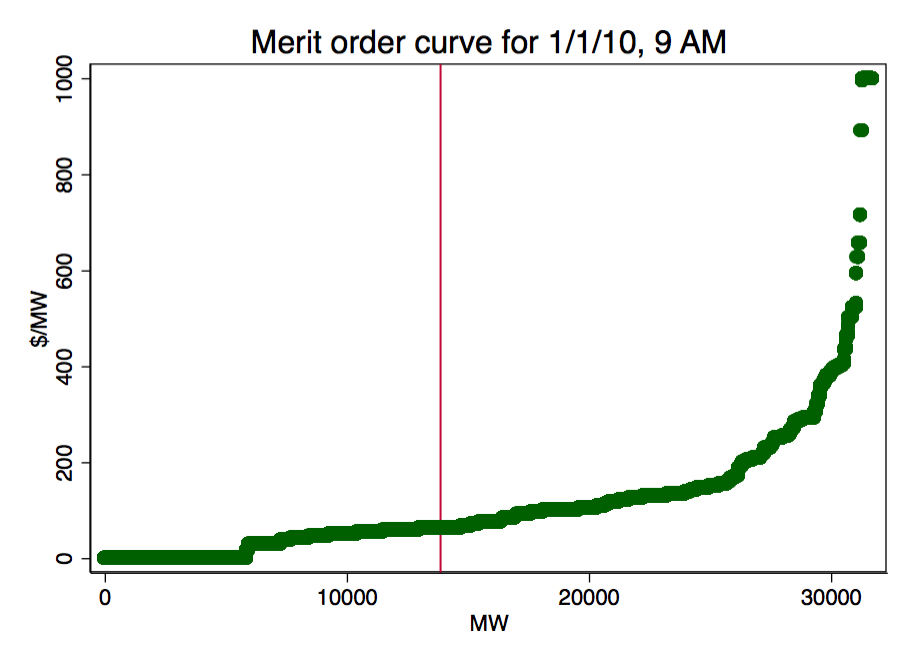
\includegraphics[width=12cm]{figures/bid2010}
    \floatfoot{Figure 7: The slope of the bid curve is determined by generator's marginal costs.}
\end{figure}

\subsection{Interaction of supply and demand}
The difference between the two curves emphasizes the importance of the energy mix on price outcomes - the shape of the supply curve directly determines price and price stability, mapping each level of demand to price. Holding demand fixed, the two changes in the supply curve that can lead to an increase in clearing price are 1) the increase in price of any generation to the left of demand to a price above the clearing price, and 2) the exit of any generation to the left of demand. Similarly, clearing price decreases in the case that 1) the decrease in the price of any generation to the right of demand to a price below the clearing price, and 2) the entry of any generation to the left of demand. Renewable resources like wind bidding in at \$0.00 decrease price through the second condition, pushing all other bids to the right.

However, shifts in demand confound the effects of these changes in the supply curve by changing the intersection at which the clearing price is found. In order to know that an increase in wind generation as we model results in a decrease in the clearing price, the following must be true: 1) wind does not cause the price of any generation to the left of demand to increase to a price above the clearing price, and 2) wind does not cause the exit of any generation to the left of demand. We can assume that neither of these effects occur as a result of strategic action due to the role of the IMM in preventing anti-competitive behavior. Thus, the only other cause of this would be the existence of some characteristic of wind generation that directly causes increases the price of other generation below the clearing price, and/or causes the exit of generation below the clearing price. This is not to be confused with an omitted exogenous factor that causes both an increase in wind and one of the above effects. Such an omitted variable could be cold weather, which increases mean wind output and also indirectly increases the price of natural gas generation through higher fuel costs because of high demand for natural gas as a heating fuel. However, this is not a causal relationship. I assume in my methodology that there are no direct, causal effects of increased wind generation on changes in other generators' prices or quantities.

\subsection{Effect of wind}
Since wind bids in at \$0.00 (or below down to -\$150.00, the minimum allowable price), it shifts the bid curve to the right by the magnitude of its quantity. This is notably equivalent to reducing demand by the same magnitude, since supplying at \$0.00 is effectively the same as negating demand in terms of setting the clearing price. Thus, if additional wind bids have no effect on the rest of the bid curve as assumed, it should always suppress the price. There may be changes in supply composition in the long run -- if generators exit because they are priced out of the market and are unable to sustain themselves through capacity payments -- but this effect is unquantifiable due to a lack of extensive data on generator exit (see Part V for a longer discussion).

The distance between the two curves in the graph below at their points of intersection with demand is the price change that occurs with the addition of 5,000 MW of wind generation.

\begin{figure}
    \centering
    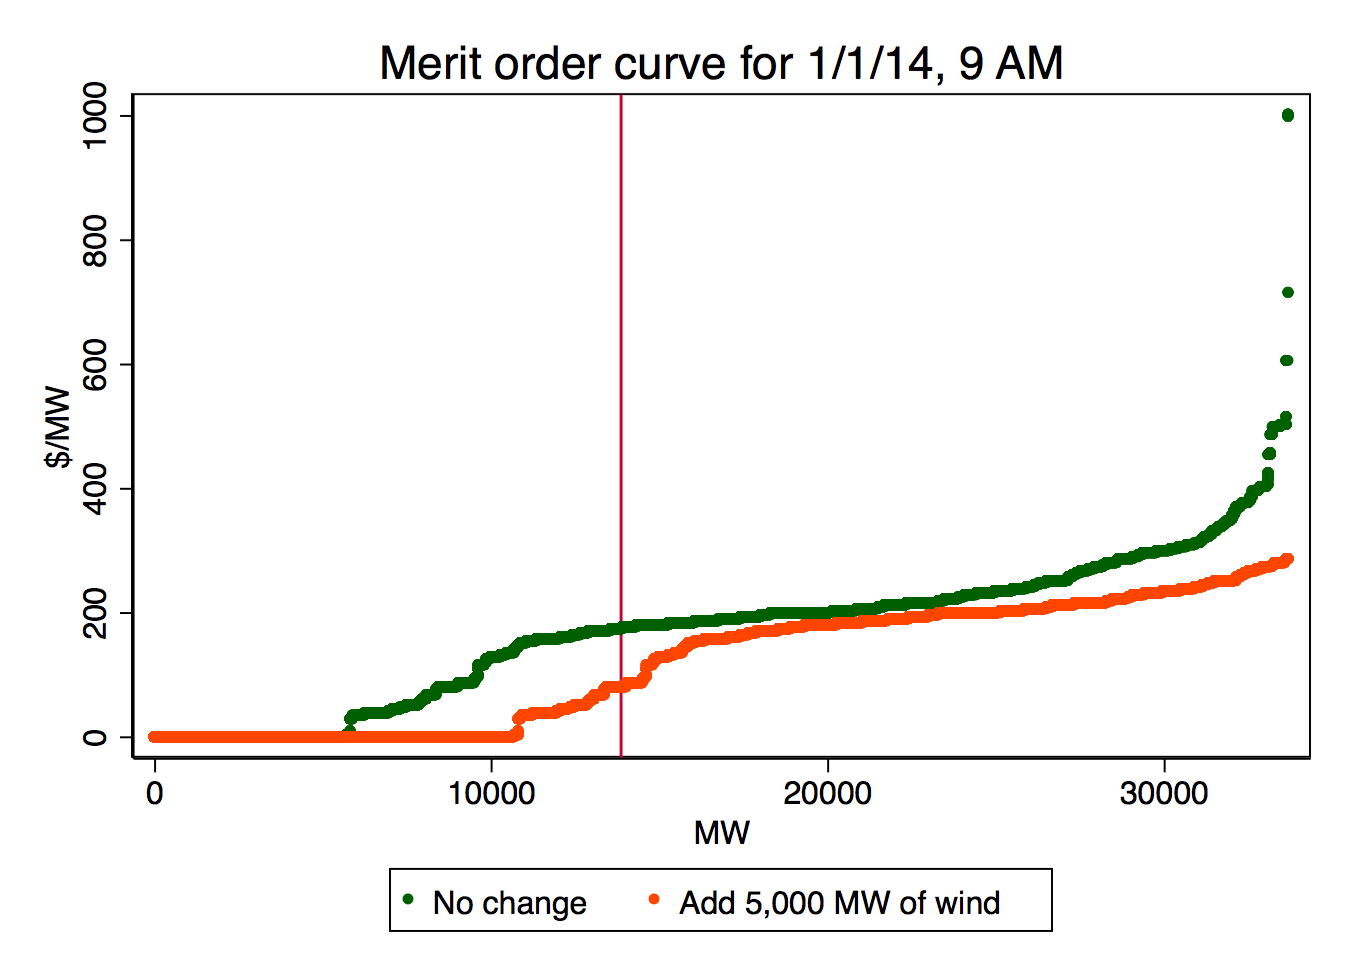
\includegraphics[width=12cm]{figures/add5000mw.jpg}
    \floatfoot{Figure 8: Adding wind to the system shifts the bid curve to the right.}
\end{figure}


\section{Historical Relationships Between Resource and Price}
Before conducting a simulation of the day-ahead market under different scenarios of increased wind penetration, it is useful to look at the historical relationship between wind (and each other resource) with price in order to get a sense of each resource's relative marginal impact on clearing price. With historical data from ISO-NE's day-ahead market on the years 2010-2014, it is possible to estimate the relative magnitudes of each resource's effects on clearing price by regressing price on its share of hourly supply. This reveals the relative marginal costs of each resource, which can be ordered along the merit curve based on the magnitudes and signs of their coefficients.

\subsection{Data}
Data on the resource mix comes from the ISO's daily reports of generation by fuel type, which provides the daily total MW contribution of each of the following resources: coal, gas, hydro, nuclear, oil, refuse, solar, and wind. [data2] This includes the energy in the day-ahead and real-time markets and contracts. I focus only on the day-ahead market, but the inclusion of the other two should not have a significant impact on the mix: only the day-ahead and real-time function as markets that update in the short run, while contracts hold on a longer timescale. Between the markets, day-ahead supply accounts for 30-40\% of supply while real-time accounts for the remaining 0-10\%. Whether the resource mix differs significantly between the two markets is undetermined because of the lack of distinction between their shares of total supply; without a means of accounting for any difference with the data, I assume that they do not. However, even if the mix differed significantly between the two markets, the real-time would have a smaller impact on the mix because of its smaller share of total supply. [7]

Data on hourly market conditions comes from the ISO's yearly zonal information reports [data1]. They include hourly information for each day of the year on characteristics such as day-ahead energy cost, temperature, and day-ahead demand (the three factors I use in the regression to follow). To match the observation timescale of the resource mix data, I average these variables to the daily level.

The US Energy Information Administration provides information on natural gas prices at the daily level via the Henry Hub Natural Gas Spot Price, which functions as the pricing point for natural gas futures contracts traded on the New York Mercantile Exchange (NYMEX). These prices are measured in dollars per million Btu, and are the most standardly used measure of natural gas prices. [data4] 

\subsection{Regression}
To estimate the impact of each resource on price, I regress the daily average day-ahead price $P_{t}$ on each resource's share of daily supply, $R_{it}$ for resource i, controlling for daily average day-ahead demand $D_t$ and the price of natural gas $G_t$. The observations are at the daily timescale, for each day of 2010-2015.

\begin{equation}
P_{t} = \beta_0 + \bigg( \sum_{i=1}^{r} \beta_{it}R_{it} \bigg) + \beta_8D_t + \beta_9G_{t} + \varepsilon_{t}
\end{equation}

I use a resource's share of supply (multiplied by 100) $R_{it}$ rather than its absolute quantity, so that the coefficient may be interpreted as the effect of increasing its share of total supply by 1\%. Season-year fixed effects (i.e. one group is the fall of 2010, another is winter of 2010-11) control for variation from other system-wide trends, such as entry and exit of suppliers, changes in market rules, and other factors that may not be immediately obvious. Day-ahead demand controls for variation in price resulting from changes in the level of demand; the fact that demand is exogenous to price and thus a valid control follows from the assumption that it is perfectly inelastic to price. The price of natural gas controls for its exogenous effect on clearing price, which may otherwise confound the effect of natural gas's share on price (as natural gas is more expensive but appears in smaller quantities during the winter, and less expensive but appears in greater quantities in the summer, biasing its effect in a negative direction) as well as the coefficients of any other resources exhibiting seasonal variation.

The magnitudes of the effects are likely weakened by the averaging of hourly data up to the daily level for each observation. The ability to look at data at the hourly level would more accurately correlate more granular spikes and dips in price with changes in the resource mix. Additionally, the resource mix represents the system resource mix rather than solely the day-ahead energy mix. However, the day-ahead market (30-40\% of supply) determines nearly all marginal change in the resource mix, since contracts (60\% of supply) last for multiple years and the real-time market (0-10\% of supply) accounts for a negligible amount of procurement \parencite{christophergeissler2016}.

regression output goes here: the whole resource mix

Coal has a highly positive and statistically significant coefficient, suggesting an increase in its supply share always contributes to higher clearing prices, as expected. A resource on its way out due to changing environmental policies and technological advancements, coal continues to exit the market, replaced by natural gas, (another quickly-ramping fossil fuel resource, but with lower emissions) \parencite{isonewengland2015outlook}. Its use peaks in the winter to cover demand that cannot be satisfied by natural gas during those months.

Though their coefficients are not statistically significant, hydro, refuse, and solar are, as expected, price suppressors as renewable fuels with low to no marginal cost.

Nuclear has a significant, negative coefficient. Though technically not renewable, it bids in near zero as renewables do and pushes more expensive generation out of the system, acting as a price suppressor. It is a ``must-run'' resource that has high start-up and shutdown costs, and low marginal cost, acting as a constantly-supplying baseload fuel. 

Oil has the most highly positive coefficient since it is generally the highest cost fuel in the market, appearing at the rightmost part of the bid curve and always setting the clearing price when it contributes to supply. Its use peaks in the winter to fill in demand that is left unsatisfied due to winter natural gas shortages. Though it contributes an average of 0.584\% of supply, it has a significant effect (unlike the higher-penetration renewables mentioned above) because of its role as a price setter at the top of cleared supply.

From the larger regression, wind appears to have a positive coefficient at the 92\% confidence level. This is counterintuitive -- as wind bids in around \$0.00 (or below), which should give it a price suppressant effect and contrary to the findings of other researchers' results in similar analyses.

regression output goes here: wind by season

An inspection of wind's effect at the seasonal level reveals extremely different outcomes by season. Spring and summer appear largely indeterminate from fall (the omitted season), but the coefficient of winter appears to be extremely large and significant. Holding to the assumption that strategic bidding does not occur in response to wind generation, I posit that there must be some confounding factor responsible for both increases in wind generation in the winter and clearing price. Wind has both its greatest mean and standard deviation in the winter, as colder weather strongly correlates to increased but more variable wind generation. The use of temperature as an additional control does not seem to impact the high coefficient of winter-wind, suggesting that the coldness of the weather itself is not to blame. One possible explanation may be that the merit order becomes violated more often as wind variability increases, due to the need to quickly fill in supply gaps that result from inaccurate wind forecasts; this would hypothetically be done by calling upon quick-starting but more expensive resources like oil or natural gas. However, the frequency at which these merit order violations occur is difficult to discern from our data. 

The fact that the effect of wind on price has been shown to be negative in other markets showing similar seasonal variability (eg. Germany [23]) suggests that this positive effect may be specific to this regression estimation or the New England market. Assuming that the highly positive coefficient does not imply a causal relationship between wind generation and high prices, the simulation results should still hold; however, if a causal relationship can be shown, the cause must be incorporated or else the results will be biased in the negative direction.

regression output goes here: gas by season

Natural gas has been omitted from the regression to avoid collinearity, and was chosen because of its general role as the market's marginal fuel, setting the clearing price in most hours. However, a look at its effects on price by season reveals seasonal fluctuations. 

Natural gas has a negative coefficient as a fuel comprising the gradually sloped middle of the bid curve, meaning that it is likely often but not always the marginal generator. It makes up a smaller share of generation in extreme price events (when the sharply sloped right side of the curve enters into the supply share) as a middle fuel, and generally sets prices around the average price, thus having a net price suppressant effect. It exhibits a more highly negative in the winter because it is used less often to satisfy winter peaks. This is due to gas' higher demand as a heating fuel in the colder winter months, which causes the price of gas generation to spike and makes it less economical than coal and oil \parencite{isonewengland2015outlook}. Thus, when clearing prices are the highest in the winter from increased coal and oil use, gas supply is lowest. The opposite occurs in the summer, where it is used to satisfy a large percentage of peak demand, which then is cleared by more expensive fuels.

\section{Checking For Strategic Behavior}
A hypothetical way in which other generators may manipulate price in the face of increased wind generation (as predictable from publicly accessible wind forecasts) is by decreasing the quantity of generation that they bid in order to increase the clearing price that results. If this type of manipulation occurs, there should be a negative relationship between the amount of wind generation and the amount of non-wind generation. I check this by regressing the total supply offered at price greater than zero on the amount of wind contributing to system supply on a given day. Note that supply for nonzero price is a proxy for non-wind generation, since we cannot identify individual bids in our dataset by their resource type; this comes at the cost of excluding other renewable generation or nuclear generation from the non-wind supply as well, since those resources can also bid in at \$0.00. However, we have no reason to believe that resources near the leftmost side of the bid curve priced near wind would have any incentive to strategically alter quantity, as near-certain price takers.

regression output goes here: nonWindBids (don't have data so need to copy to table)

We see a positive but statistically insignificant coefficient on wind above, giving no reason to suspect that manipulative quantity withdrawal occurs. It is interesting to note that temperature is a large contributor to the amount of supply available to the system; a likely explanation for this trend is the cost of cooling most generation plants (particularly coal, oil, natural gas, and nuclear). In warm weather, it becomes more costly to generate the same amount of energy because of increased cooling costs from the effects of ambient heat, whereas the opposite effect occurs for cooler temperatures \parencite{worldnuclearassociation2015}. 

\section{Simulating Increased Wind Penetration}
In order to determine the clearing prices that would have resulted from adding various amounts of wind generation into historical data hours, I run a simulation in Python which takes hourly data from ISO-NE on day-ahead market energy offers and demand from 2010 to 2014, constructs supply curves from the energy offers, and calculates clearing prices based on the intersection of the supply curve with the fixed hourly demand, as seen in the representation above. The original clearing price  for the hour is first calculated by intersecting demand with the original set of energy offers. Then, to calculate the prices that result from additional wind generation, I modify the supply curves of each hour to add wind bids in increments of 100 MW (greater granularity makes the datasets too large to process without providing much additional information), and then re-solve for the supply-demand intersection to find the new clearing prices at each of these increments. 

Re-solving problem after inserting an additional wind bid is equivalent to decreasing demand: shifting the entire bid curve to the right by inserting 1 MW of wind at the bottom of the merit order is equivalent to shifting demand down by 1 MW in terms of the clearing price resulting from the new intersection of supply and demand. Thus, I decrement demand rather than resolving the problem at each step with a new supply curve in order to reduce computational complexity.

I assume that wind bids in at \$0.00 in constructing this simulation. Though in reality wind also bids in at negative prices (frequently dropping to the minimum allowable price of -\$150), this is irrelevant to my construction as I do not add enough wind energy for price to fall beyond \$0.00 and thus allow for the difference between a \$0.00 bid and a negative bid to take an effect. Most of the variation in price change that we seek to describe comes from the replacement of generators (such as gas and coal) bidding in at higher, clearly positive prices at the rightmost side of the bid curve.

Depending on how far the bid curve gets pushed to the right (the ``shift'') and the nature of the price jumps between generators at the region of the curve with the marginal generator (``jump''), the change in clearing price varies as demand is held constant. I assume, in holding demand constant, that demand is perfectly inelastic to these changes in clearing price. As mentioned earlier, the elasticity of demand of residential electricity price in New England is estimated to be about -0.192 in the short run and -0.325 in the long run (Bernstein and Griffin, 2006), but the relationship between day-ahead wholesale market clearing prices and residential electricity price is unclear; energy generation (as procured through the wholesale market) is estimated to make up 65\% of electricity rates in the US (with distribution and transmission comprising the rest). Since the effect is generally small and the relationship between wholesale prices and residential rates uncertain, I assume perfectly inelastic demand in the simulation. This means that price reductions may be smaller in magnitude than our predictions may suggest \parencite{usenergyinformationadministration2015}.

Additionally, I assume that supply from other generators remains perfectly inelastic. This is certainly not true for large quantities of additional wind in the long run, as more and more generation is displaced by wind's presence at the bottom of the bid curve - some older, more expensive generation will be pushed out of the market. However, whether a generator exits depends not only on its status in the day-ahead and real-time markets, but also on the amount revenue it collects from capacity markets \parencite{isonewengland2015outlook}. Little data on the rate and cause of exit from the market is accessible, making it difficult to reasonably estimate changes in other generators' supply in response to increased wind penetration. Thus, the effect of this assumption on our results is indeterminate: if generators appearing directly above wind on the merit curve exit, price may increase in higher demand scenarios where they can no longer provide a more gradual slope on the exponential curve. But if generators appearing at the top of the curve exit because they are never activated even in the highest demand hours, this should have no additional effect on price at any level of demand.

regression output here: priceDiff thing that I have to copy over

It should be noted that the clearing prices calculated from the intersection of cleared demand and the bid curves constructed from hourly bidding data do not exactly match up with actual hourly clearing prices. This can be explained by our earlier assumption that the merit order is never violated, which does not hold true in the case that other grid constraints, such as transmission constraints, come into play. The difference between the calculated simulation price and the actual price grow with higher demand and the marginal loss component of the hour. The marginal loss component measures the cost of transmission and reserve constraints that interfere with the pure use of the merit order as the procurement process, and is not itself included in the wholesale energy cost. It is the cost of losses at a given node (location) on the grid, relative to the average of system node prices. [19] However, it correlates to high prices as it indicates there are constraints on the grid that may have caused system operators to violate the merit order and elect a more expensive generator in order to meet some other physical grid constraint \parencite{christophergeissler2016}. Temperature extremity (measured here as the absolute difference between the recorded average temperature and 50 F) seems to have the opposite effect, with more extreme temperatures decreasing the difference between the prices. The congestion component, which measures the cost of congestion on the grid, appears statistically insignificant.

Despite these differences, there is still a near 1-to-1 correlation between the prices calculated by the simulation and the actual historical system prices (regressing one price on the other gives a coefficient of 1.018), though they deviate to a greater extent at higher prices. This close relationship suggests that the merit order (as used in the simulation) generally holds, especially at average conditions. Though there is deviation from the historical prices, the shapes of the bid curves should remain the same, meaning our estimations of net price change from the simulation should remain accurate. Assuming that increased wind generation does not affect the frequency of these violations of merit order, the simulation output should generally underestimate the magnitude of net price change, since the calculated prices skew towards less extreme price spikes as compared to the actual prices.

\begin{figure}[bp!]
    \centering
    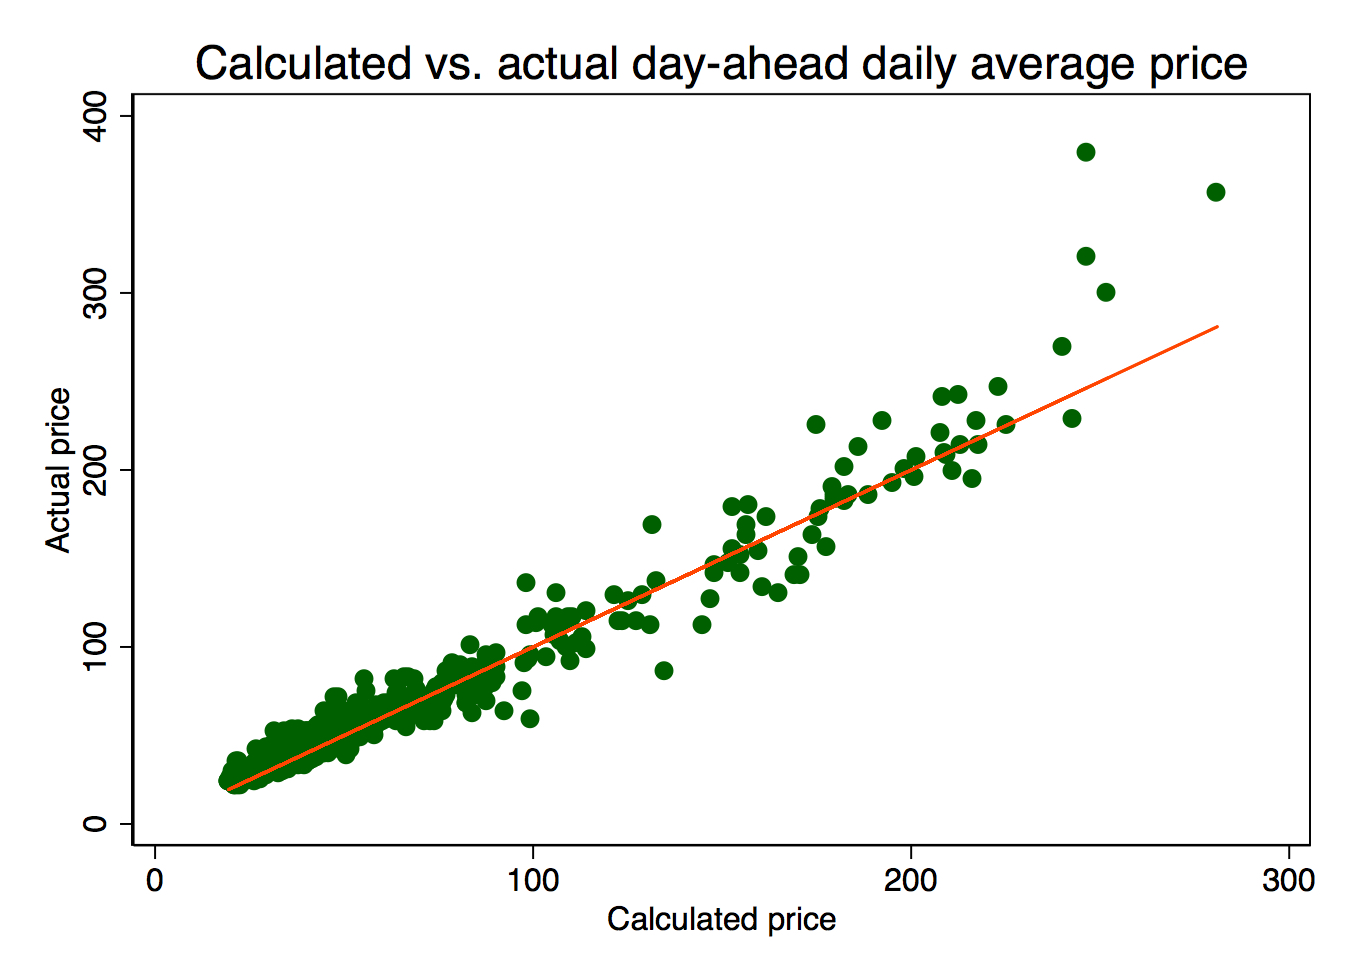
\includegraphics[width=10cm]{figures/actual-calculated-diff.jpg}
    \floatfoot{Figure 9: The difference between the calculated and actual price differs the most during price spikes. The orange line represents a 1-to-1 relationship.}
\end{figure}

\begin{figure}[bp!]
    \centering
    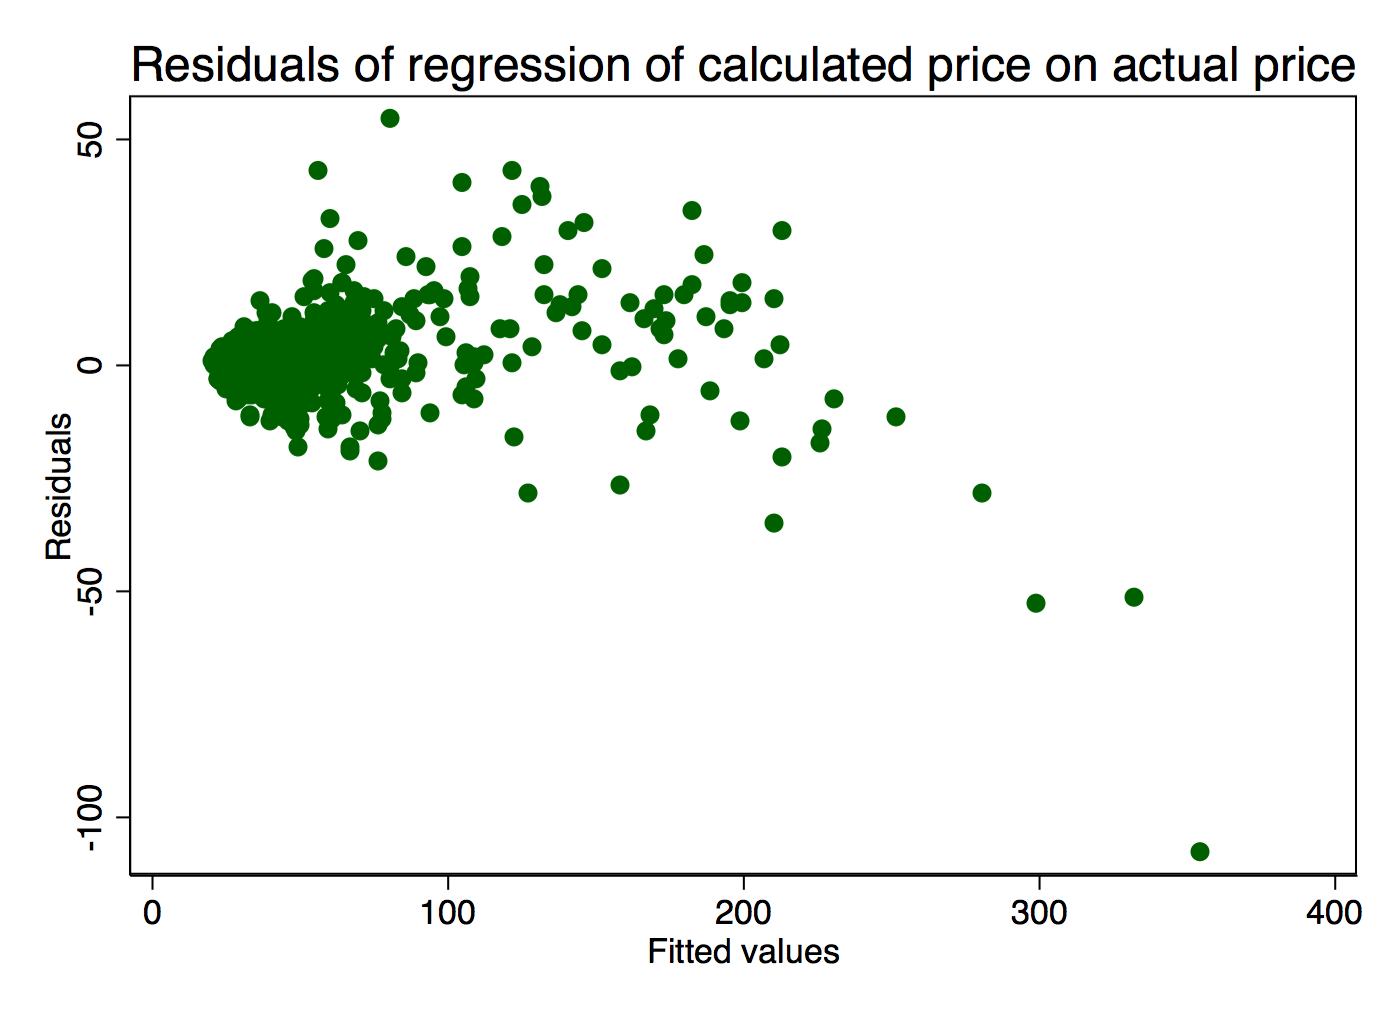
\includegraphics[width=10cm]{figures/calc_actual_residuals.jpg}
    \floatfoot{Figure 10: Calculated price skews too low as actual price increases.}
\end{figure}


\pagebreak

\section{Simulation Results}
Running the simulation, we see very different levels of price change depending on the demand and resource mix present in a given hour. During high demand hours, there are more immediate and steep drops in price as generation is added, due to the exponential shape of the merit order curve. In fact, the shape of the price change curve for additional wind is exactly the same as the merit order curve (up to its intersection with demand) flipped horizontally. This can be seen in the graphs below:

\begin{figure} [h!]
    \centering
    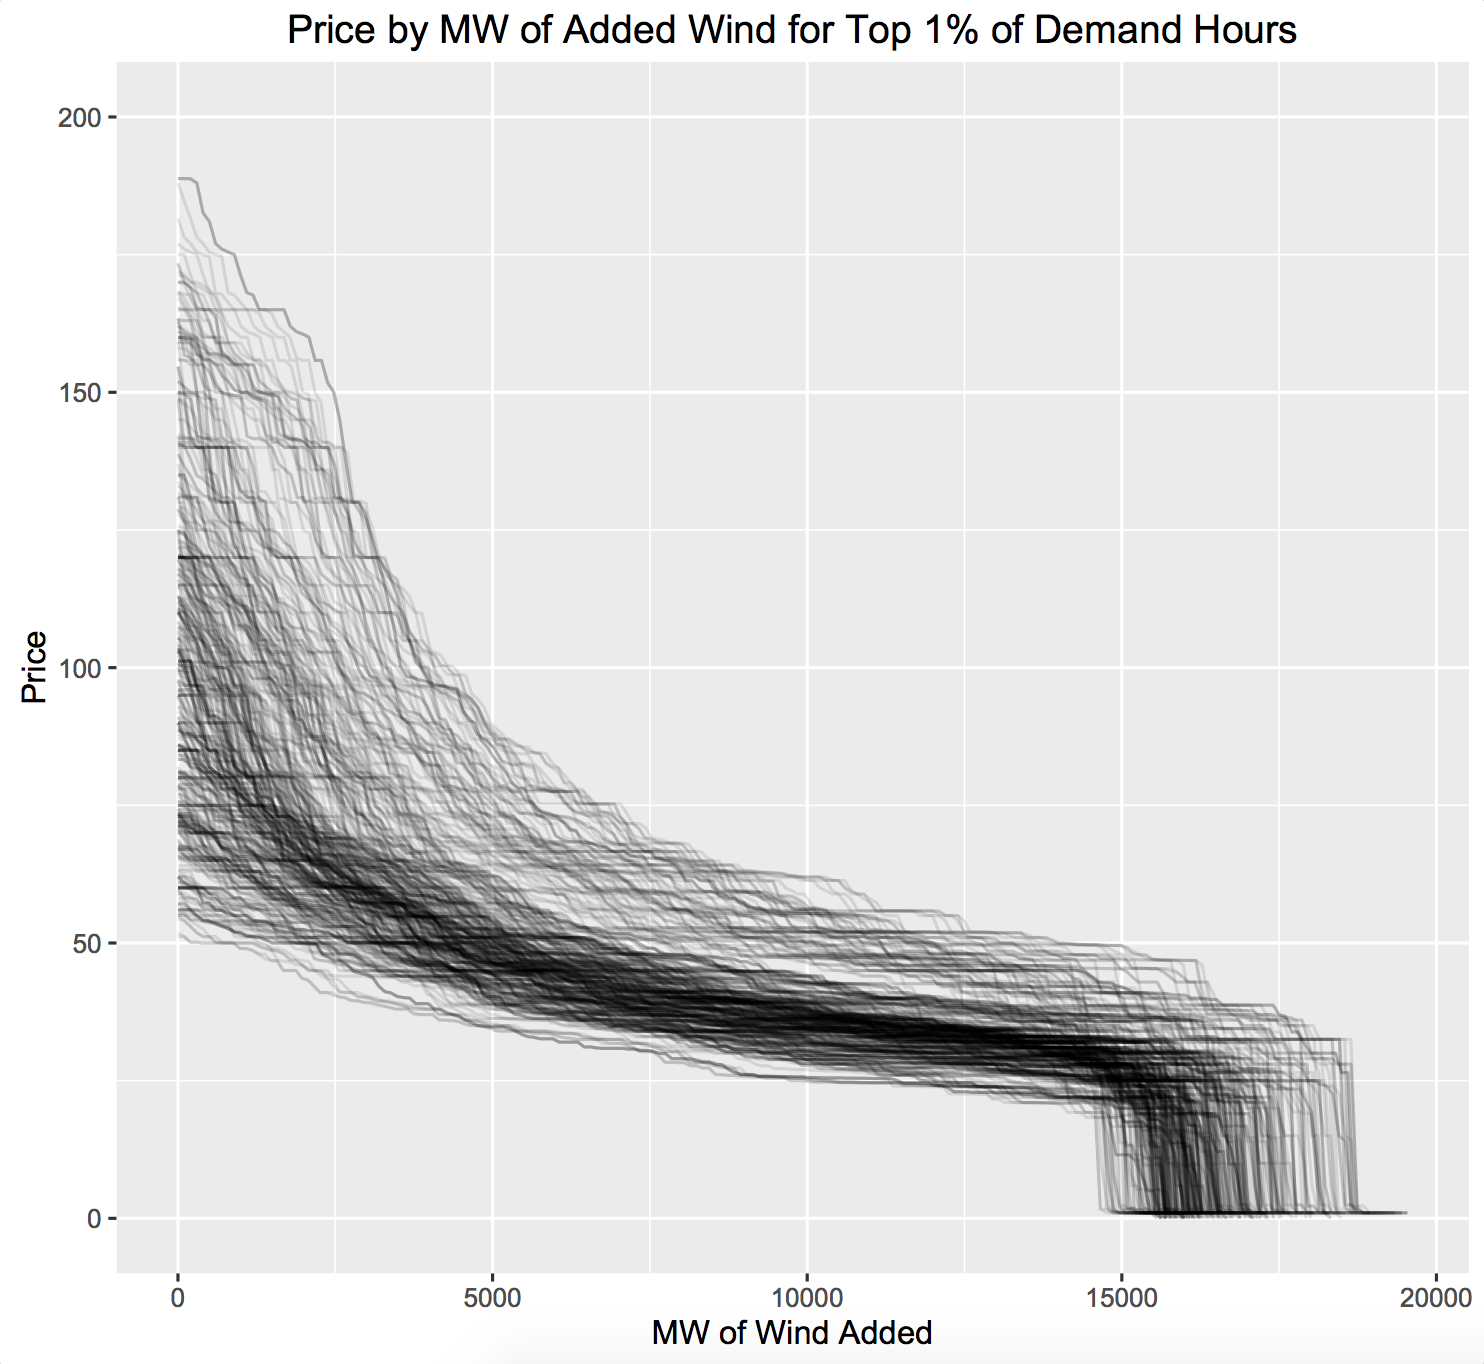
\includegraphics[width=13cm]{figures/top1wind}
    \floatfoot{Figure 11: Price decreases sharply with additional wind during high demand hours.}
\end{figure}

\newpage

\begin{figure}[h!]
    \centering
    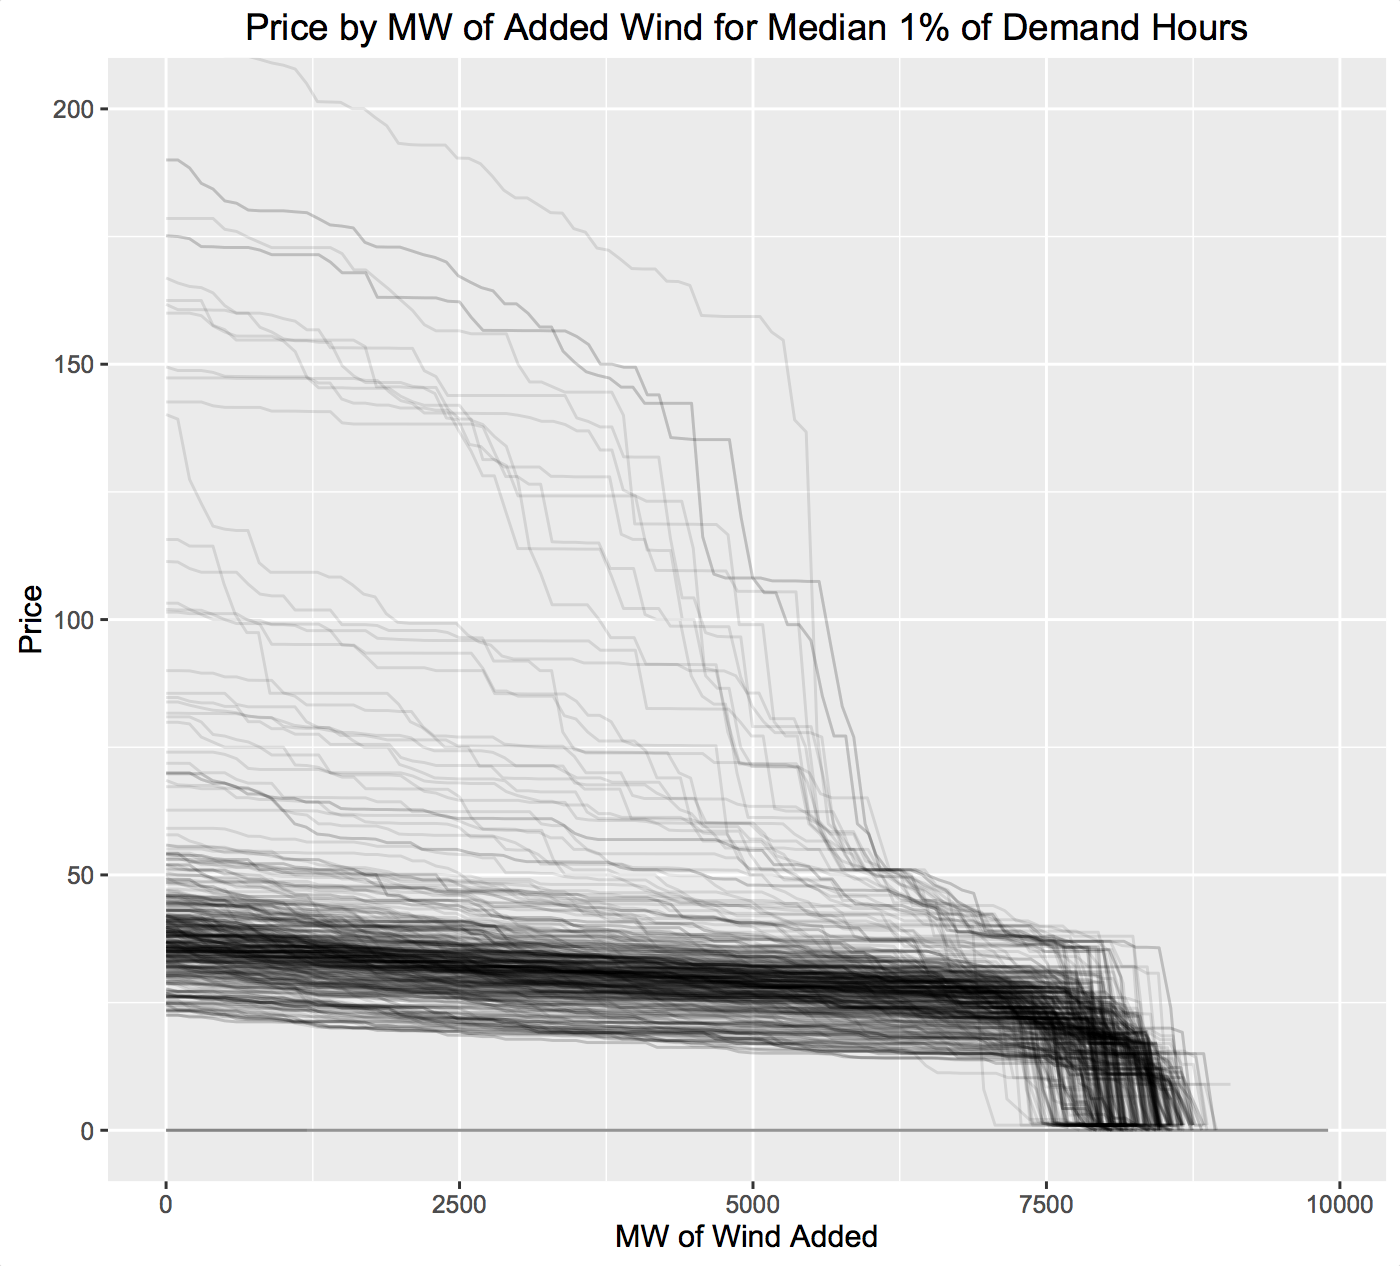
\includegraphics[width=13cm]{figures/med1wind}
    \floatfoot{Figure 12: The gradual slope of the curve reflects the gradual upward slope of the middle of the bid curve, which is dominated by similarly-priced gas generation.}
\end{figure}

\begin{figure}[h!]
    \centering
    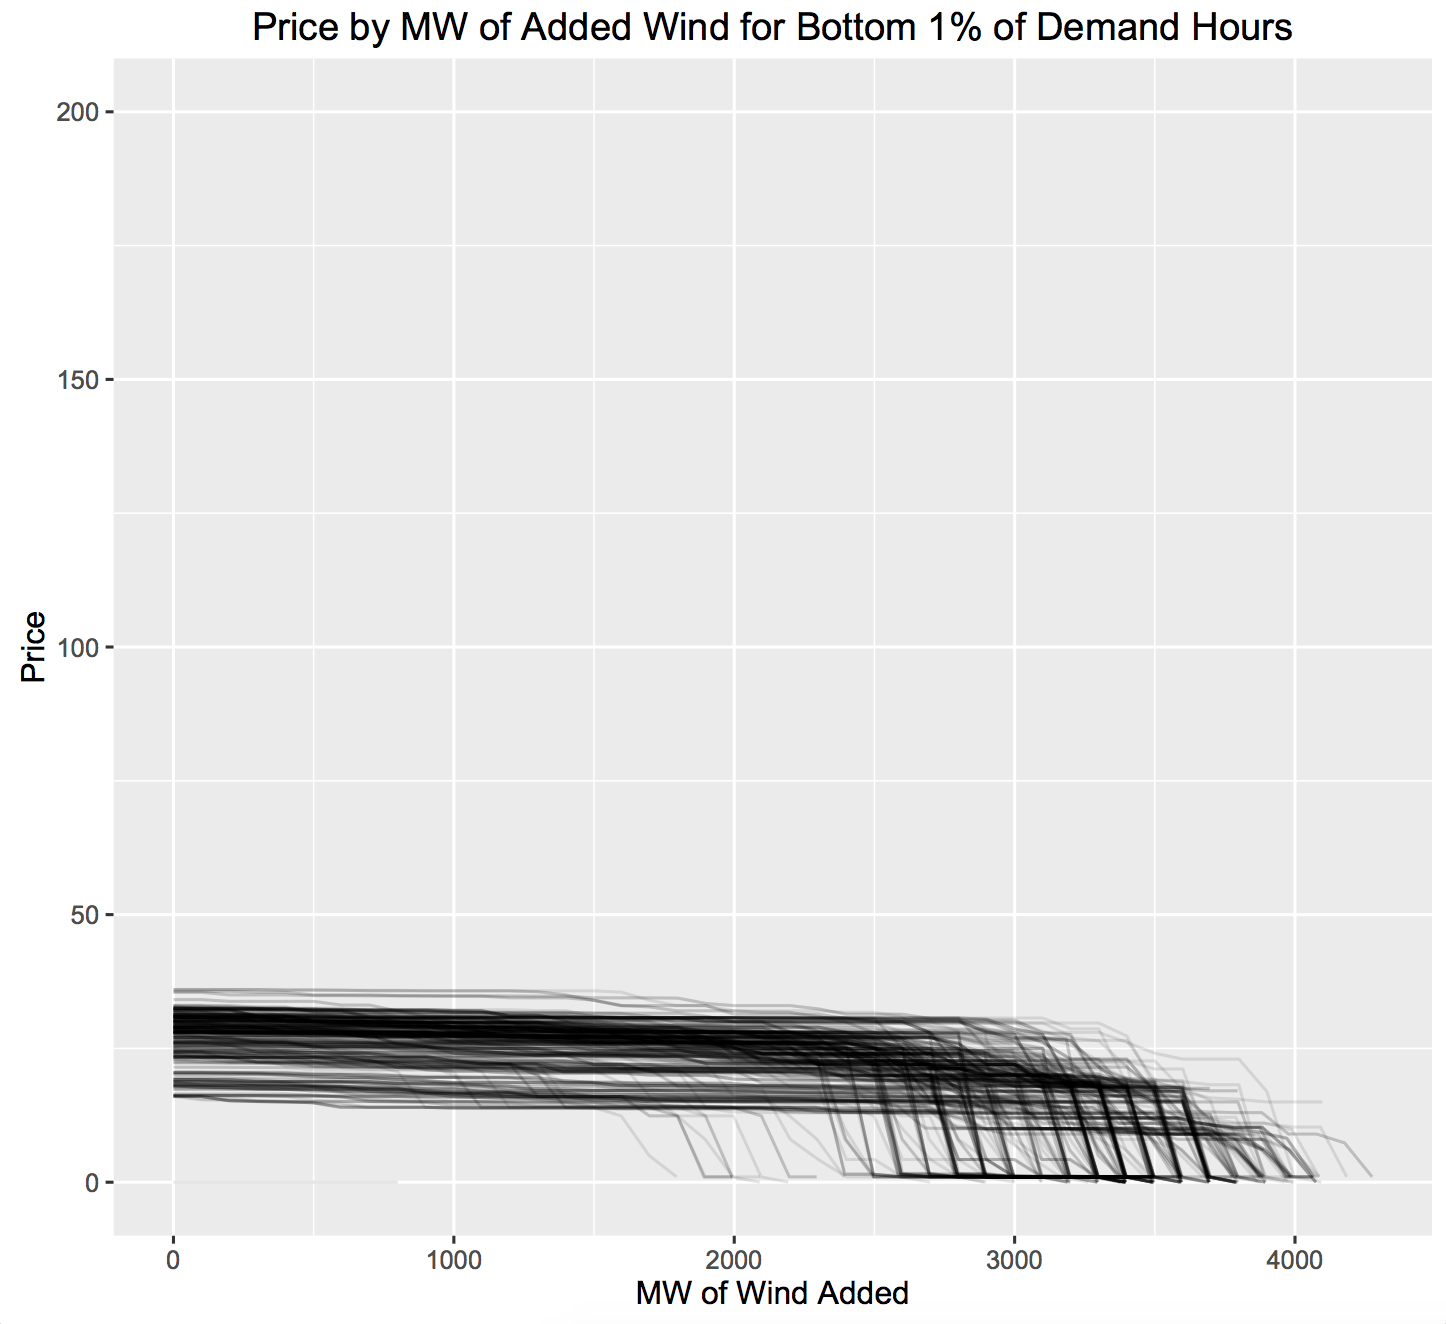
\includegraphics[width=13cm]{figures/bottom1wind}
    \floatfoot{Figure 13: At low demand, price remains steady in the face of additional wind generation.}
\end{figure}

\newpage

Given the predicted prevalence of gas and wind generation on the system as the two dominant resources of New England's future grid, I look specifically at the magnitudes of price changes under different quintiles of demand and natural gas' percent contribution to system supply. This is calculated by regressing the effect of varying MW of additional wind added to the system $W_{m}$ on net price change $\Delta P_m$ under different levels of gas penetration (g) and demand (d), the result of which is then multiplied by 100 to give a better sense of the savings in more realistically large increments. This results in coefficients that measure the average effect of an increase in wind among different conditions on the 43,800 observed hours. 

\begin{equation}
\Delta P_m = \sum_{}^{r} \bigg[ \beta_{0r} + \beta_{1r}W_{m} + \big[\sum_{}^{d} \big(\sum_{}^{g} \beta_{rdg}W_{m} \big) \big] + \varepsilon_{rm} \bigg]
\end{equation}

To give a sense of prices as they were before additional wind was added, below is a table summarizing prices at each of the demand quintiles that hours are sorted into, followed by the results.

\begin{center}
\begin{tabular}{ |p{5cm}||p{5cm}|p{5cm}|p{5cm}|  }
 \hline
Demand & Mean price (\$/MW)\\
 \hline
Bottom 25\% (Q1) & \$33.339 \\
 \hline
Lower middle 25\% (Q2) & \$43.001 \\
 \hline
Upper middle 25\% (Q3) & \$46.951 \\
 \hline
Top 25\% (Q4) & \$69.940 \\
 \hline
Top 5\% & \$73.029 \\
 \hline
Top 1\% & \$99.404 \\
 \hline
\end{tabular}
\end{center}

%first
 \begin{center}
\begin{tabular}{ |p{2.5cm}||p{3.4cm}|p{3.4cm}|p{3.4cm}|  }
 \hline
 \multicolumn{4}{|c|}{$\Delta$ in price per 100 MW added, for 0-1,500 MW of additional wind} \\
 \hline
Demand & Low gas (g$\leq$42.1\%) & Median gas (4.21\%$<$g$\leq$53.4\%) & High gas (g$>$53.4\%) \\
 \hline
Q1 & -\$0.268 & -\$0.146 & -\$0.121 \\
 \hline
Q2 & -\$0.366 & -\$0.218 & -\$0.188 \\
 \hline
Q3 & -\$0.398 & -\$0.261 & -\$0.243 \\
 \hline
Q4 & -\$0.658 & -\$0.437 & -\$0.505 \\
 \hline
Top 5\% & -\$1.681 & -\$0.694 & -\$0.777 \\
 \hline
Top 1\% & -\$1.218$\dagger$ & -\$1.218 & \it{-\$1.334 (P=0.004)} \\
 \hline
\end{tabular}
\end{center}
\small
$\dagger$ = collinear with the median gas value\\
Each one of these coefficients has P=0.00 except for the italicized entries, which have their P-value written beside them.

%second
 \begin{center}
\begin{tabular}{ |p{2.5cm}||p{3.4cm}|p{3.4cm}|p{3.4cm}|  }
 \hline
 \multicolumn{4}{|c|}{$\Delta$ in price per 100 MW added, for 1,500-3,000 MW of additional wind} \\
 \hline
Demand & Low gas (g$\leq$42.1\%) & Median gas (4.21\%$<$g$\leq$53.4\%) & High gas (g$>$53.4\%) \\
 \hline
Q1 & -\$0.382 & -\$0.170 & -\$0.208 \\
 \hline
Q2 & -\$0.431 & -\$0.176 & -\$0.128 \\
 \hline
Q3 & -\$0.368 & -\$0.206 & -\$0.173 \\
 \hline
Q4 & -\$0.528 & -\$0.337 & -\$0.382 \\
 \hline
Top 5\% & -\$0.904 & -\$0.542 & -\$0.587 \\
 \hline
Top 1\% & -\$0.965$\dagger$ & -\$0.965 & \it{-\$1.036 (P=0.040)} \\
 \hline
\end{tabular}
\end{center}

%third
 \begin{center}
\begin{tabular}{ |p{2.5cm}||p{3.4cm}|p{3.4cm}|p{3.4cm}|  }
 \hline
 \multicolumn{4}{|c|}{$\Delta$ in price per 100 MW added, for 3,000-5,000 MW of additional wind} \\
 \hline
Demand & Low gas (g$\leq$42.1\%) & Median gas (4.21\%$<$g$\leq$53.4\%) & High gas (g$>$53.4\%) \\
 \hline
Q1 & -\$0.725 & -\$0.491 & -\$0.433 \\
 \hline
Q2 & -\$0.784 & -\$0.172 & -\$0.131 \\
 \hline
Q3 & -\$0.449 & -\$0.156 & -\$0.119 \\
 \hline
Q4 & -\$0.519 & -\$0.238 & -\$0.258 \\
 \hline
Top 5\% & -\$0.689 & -\$0.364 & \it{-\$0.383 (P=0.001)} \\
 \hline
Top 1\% & -\$0.686$\dagger$ & -\$0.686 & -\$0.655 (P=0.138) \\
 \hline
\end{tabular}
\end{center}


Among these estimations of wind's effect on prices at different levels of increased wind, demand, and contribution of gas to total supply, a few trends reveal themselves. First, price change becomes greater at all levels of gas penetration as demand rises for low and medium (<=3,000 MW) additions of wind. Second, the magnitude of price change increases with greater levels of gas penetration for low and medium additions as well. This is likely because gas takes a larger share of supply when both demand and prices are high; high gas share suggests that demand may have cleared at a part of the bid curve where prices display a steeper slope. High additions of 3,000-5,000 MW do not follow these trends, as prices have already fallen down the steepest decline in the bid curve, which is then followed by a relatively flat region of similarly priced gas generators. Results suggest that hours at which the greatest price decreases can be realized are those with a high share of gas generation and high demand, with the most negative coefficient appearing as -\$1.334 per 100 MW for penetrations of gas over 53.4\% at the top 1\% of demand hours.

\begin{figure}
    \centering
    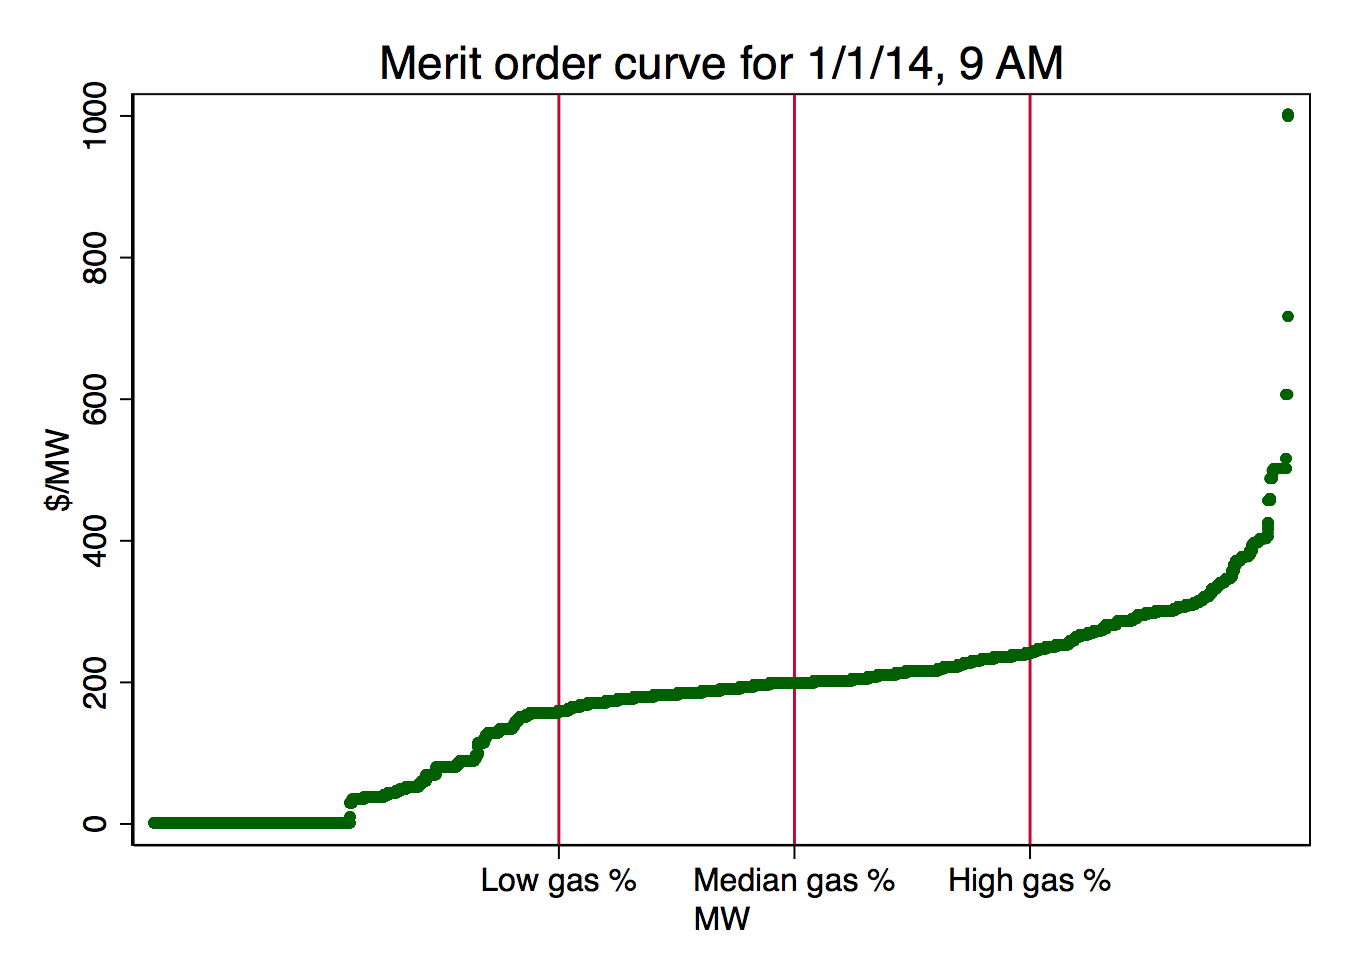
\includegraphics[width=12cm]{figures/low-med-high-gas}
    \floatfoot{Figure 14: The red lines designate different levels of demand at which gas contributes varying levels of supply.}
\end{figure}

It should be noted that these effects may vary as the generation mix changes. Higher penetrations of gas suggest that a high amount of other highly-priced (and likely higher priced) resources are also being called upon. If we expect these highly-priced generators to exit the market upon being priced out by additional wind generation, then price changes should occur as generally predicted. However, if for some reason generation in the middle of the curve exited the market rather than price-clearing marginal generation, price savings may not be as high as anticipated. 

The assumption of fixed supply should not have an impact on our results as long as generators at the margin are the ones exiting, as discussed above. But the assumption of perfectly inelastic demand may not completely hold in the long run, meaning that demand may rebound in the face of lower prices brought on by changes in the generation mix. However, these will likely still be small in the face of other drivers of future demand, one major source being the increased use of electric vehicles.

It is also important to realize in interpreting this simulation that an additional MW of wind generation capacity on the system does not translate into a constantly available MW of wind generation, as wind is a source of variable generation relying on the weather. How often a turbine runs and the magnitude of its output depends on its location, but the average turbine produces electricity 70-85\% of the time, with output depending on wind velocity. More than 1,000 MW of additional wind capacity would need to be built for 1,000 MW to constantly be available on the system. [25] 

As New England's generation mix becomes increasingly dominated by wind and natural gas, the bid curve will gradually lose its exponential peak and display more of a logarithmic shape, with a long stretch of \$0.00/MW bids followed by a step up to a steady stretch at the price of natural gas generation. In this largely dual-fuel paradigm, prices should remain relatively stable, switching between the two levels of price depending on demand.

\section{Conclusion}
By simulating the direct effect of increased wind supply on ISO-NE's day-ahead electricity market, I have created estimations of the effects of different levels of additional wind on the market clearing price, as varying by the level of demand and share of supply provided by natural gas. These have shown that that reductions in price are greatest when the percentage share of natural gas and level of demand are very high, due to the steepness of the rightmost side of the bid curve which is accessed under these conditions. Regressing the effect of each type of generation in the market on historical clearing prices provided insight on the ordering of these resources in the merit order, as well as on their relative marginal impacts on the clearing price. 

Though wind's share of supply in New England is currently still small, providing only about 1\% of supply on average, this is set to change. State-sponsored programs, federal subsidies, tax credits, and falling technology costs have made wind one of the fastest growing resources in the world at a time when reducing emissions from the power sector is more important than ever \parencite{isonewengland2015outlook}. With more than 4,000 MW of proposed wind projects currently under consideration by ISO-NE, such savings in energy cost for the grid are soon to come. [24] \nocite{*}

\pagebreak
\printbibliography


\pagebreak
\section*{Appendix}
\setcounter{table}{0}
\renewcommand{\thetable}{A\arabic{table}}


\pagebreak
\pagebreak
\end{document}
\end{document}